% Options for packages loaded elsewhere
\PassOptionsToPackage{unicode}{hyperref}
\PassOptionsToPackage{hyphens}{url}
%
\documentclass[
]{book}
\usepackage{lmodern}
\usepackage{amssymb,amsmath}
\usepackage{ifxetex,ifluatex}
\ifnum 0\ifxetex 1\fi\ifluatex 1\fi=0 % if pdftex
  \usepackage[T1]{fontenc}
  \usepackage[utf8]{inputenc}
  \usepackage{textcomp} % provide euro and other symbols
\else % if luatex or xetex
  \usepackage{unicode-math}
  \defaultfontfeatures{Scale=MatchLowercase}
  \defaultfontfeatures[\rmfamily]{Ligatures=TeX,Scale=1}
\fi
% Use upquote if available, for straight quotes in verbatim environments
\IfFileExists{upquote.sty}{\usepackage{upquote}}{}
\IfFileExists{microtype.sty}{% use microtype if available
  \usepackage[]{microtype}
  \UseMicrotypeSet[protrusion]{basicmath} % disable protrusion for tt fonts
}{}
\makeatletter
\@ifundefined{KOMAClassName}{% if non-KOMA class
  \IfFileExists{parskip.sty}{%
    \usepackage{parskip}
  }{% else
    \setlength{\parindent}{0pt}
    \setlength{\parskip}{6pt plus 2pt minus 1pt}}
}{% if KOMA class
  \KOMAoptions{parskip=half}}
\makeatother
\usepackage{xcolor}
\IfFileExists{xurl.sty}{\usepackage{xurl}}{} % add URL line breaks if available
\IfFileExists{bookmark.sty}{\usepackage{bookmark}}{\usepackage{hyperref}}
\hypersetup{
  pdftitle={Redes multicapa como herramienta de análisis de la microbiota},
  pdfauthor={Víctor Lázaro Vidal},
  hidelinks,
  pdfcreator={LaTeX via pandoc}}
\urlstyle{same} % disable monospaced font for URLs
\usepackage{color}
\usepackage{fancyvrb}
\newcommand{\VerbBar}{|}
\newcommand{\VERB}{\Verb[commandchars=\\\{\}]}
\DefineVerbatimEnvironment{Highlighting}{Verbatim}{commandchars=\\\{\}}
% Add ',fontsize=\small' for more characters per line
\usepackage{framed}
\definecolor{shadecolor}{RGB}{248,248,248}
\newenvironment{Shaded}{\begin{snugshade}}{\end{snugshade}}
\newcommand{\AlertTok}[1]{\textcolor[rgb]{0.94,0.16,0.16}{#1}}
\newcommand{\AnnotationTok}[1]{\textcolor[rgb]{0.56,0.35,0.01}{\textbf{\textit{#1}}}}
\newcommand{\AttributeTok}[1]{\textcolor[rgb]{0.77,0.63,0.00}{#1}}
\newcommand{\BaseNTok}[1]{\textcolor[rgb]{0.00,0.00,0.81}{#1}}
\newcommand{\BuiltInTok}[1]{#1}
\newcommand{\CharTok}[1]{\textcolor[rgb]{0.31,0.60,0.02}{#1}}
\newcommand{\CommentTok}[1]{\textcolor[rgb]{0.56,0.35,0.01}{\textit{#1}}}
\newcommand{\CommentVarTok}[1]{\textcolor[rgb]{0.56,0.35,0.01}{\textbf{\textit{#1}}}}
\newcommand{\ConstantTok}[1]{\textcolor[rgb]{0.00,0.00,0.00}{#1}}
\newcommand{\ControlFlowTok}[1]{\textcolor[rgb]{0.13,0.29,0.53}{\textbf{#1}}}
\newcommand{\DataTypeTok}[1]{\textcolor[rgb]{0.13,0.29,0.53}{#1}}
\newcommand{\DecValTok}[1]{\textcolor[rgb]{0.00,0.00,0.81}{#1}}
\newcommand{\DocumentationTok}[1]{\textcolor[rgb]{0.56,0.35,0.01}{\textbf{\textit{#1}}}}
\newcommand{\ErrorTok}[1]{\textcolor[rgb]{0.64,0.00,0.00}{\textbf{#1}}}
\newcommand{\ExtensionTok}[1]{#1}
\newcommand{\FloatTok}[1]{\textcolor[rgb]{0.00,0.00,0.81}{#1}}
\newcommand{\FunctionTok}[1]{\textcolor[rgb]{0.00,0.00,0.00}{#1}}
\newcommand{\ImportTok}[1]{#1}
\newcommand{\InformationTok}[1]{\textcolor[rgb]{0.56,0.35,0.01}{\textbf{\textit{#1}}}}
\newcommand{\KeywordTok}[1]{\textcolor[rgb]{0.13,0.29,0.53}{\textbf{#1}}}
\newcommand{\NormalTok}[1]{#1}
\newcommand{\OperatorTok}[1]{\textcolor[rgb]{0.81,0.36,0.00}{\textbf{#1}}}
\newcommand{\OtherTok}[1]{\textcolor[rgb]{0.56,0.35,0.01}{#1}}
\newcommand{\PreprocessorTok}[1]{\textcolor[rgb]{0.56,0.35,0.01}{\textit{#1}}}
\newcommand{\RegionMarkerTok}[1]{#1}
\newcommand{\SpecialCharTok}[1]{\textcolor[rgb]{0.00,0.00,0.00}{#1}}
\newcommand{\SpecialStringTok}[1]{\textcolor[rgb]{0.31,0.60,0.02}{#1}}
\newcommand{\StringTok}[1]{\textcolor[rgb]{0.31,0.60,0.02}{#1}}
\newcommand{\VariableTok}[1]{\textcolor[rgb]{0.00,0.00,0.00}{#1}}
\newcommand{\VerbatimStringTok}[1]{\textcolor[rgb]{0.31,0.60,0.02}{#1}}
\newcommand{\WarningTok}[1]{\textcolor[rgb]{0.56,0.35,0.01}{\textbf{\textit{#1}}}}
\usepackage{longtable,booktabs}
% Correct order of tables after \paragraph or \subparagraph
\usepackage{etoolbox}
\makeatletter
\patchcmd\longtable{\par}{\if@noskipsec\mbox{}\fi\par}{}{}
\makeatother
% Allow footnotes in longtable head/foot
\IfFileExists{footnotehyper.sty}{\usepackage{footnotehyper}}{\usepackage{footnote}}
\makesavenoteenv{longtable}
\usepackage{graphicx,grffile}
\makeatletter
\def\maxwidth{\ifdim\Gin@nat@width>\linewidth\linewidth\else\Gin@nat@width\fi}
\def\maxheight{\ifdim\Gin@nat@height>\textheight\textheight\else\Gin@nat@height\fi}
\makeatother
% Scale images if necessary, so that they will not overflow the page
% margins by default, and it is still possible to overwrite the defaults
% using explicit options in \includegraphics[width, height, ...]{}
\setkeys{Gin}{width=\maxwidth,height=\maxheight,keepaspectratio}
% Set default figure placement to htbp
\makeatletter
\def\fps@figure{htbp}
\makeatother
\setlength{\emergencystretch}{3em} % prevent overfull lines
\providecommand{\tightlist}{%
  \setlength{\itemsep}{0pt}\setlength{\parskip}{0pt}}
\setcounter{secnumdepth}{5}
\usepackage{booktabs}
\usepackage[]{natbib}
\bibliographystyle{plainnat}

\title{Redes multicapa como herramienta de análisis de la microbiota}
\author{Víctor Lázaro Vidal}
\date{09/02/22}

\begin{document}
\maketitle

{
\setcounter{tocdepth}{1}
\tableofcontents
}
\hypertarget{resumen}{%
\chapter*{Resumen}\label{resumen}}
\addcontentsline{toc}{chapter}{Resumen}

En la biología nos vemos constantemente enfrentados a los sistemas complejos, es decir, sistemas conformados por muchos componentes que interactúan entre sí, y cuyo comportamiento solo puede ser explicado como la suma de la interacción de sus componentes. Un ejemplo de este tipo de sistemas es la microbiota, donde distintos microorganismos interactúan entre sí, con los tejidos del hospedero y con su entorno. Las redes son una herramienta matemática sumamente útil en el análisis de sistemas complejos, sin embargo el enfoque tradicional enfrenta ciertas limitaciones, pues los sistemas biológicos son sistemas dinámicos que cambian en el tiempo y en función de las condiciones. Ante tales retos, las redes multicapa se presentan como un nuevo paradigma en el análisis de sistemas complejos.

Empleando redes multiplex, analizamos bases de datos obtenidas a partir de muestras de la microbiota de dos organismos estrechamente relacionados, la solanácea \emph{Datura inoxia} y el escarabajo \emph{Lema daturaphila}. Las redes de coabundancia fueron generadas mediante los algoritmos de inferencia SparCC y ARACNe. Se hallaron comunidades bacterianas involucradas en la fijación de nitrógeno en la capa de la solanácea, mismas que podrían tener una relación mutualista con los tejidos de la planta. Tanto en la solanácea como en el escarabajo se encontraron comunidades bacterianas asociadas al tejido intestinal del insecto, lo que en la solanácea podría derivarse de la materia fecal depositada por las larvas mientras se alimentan de la planta.

Bajo el enfoque de las redes temporales, se analizaron datos de dos sujetos que experimentaron cambios en su microbiota derivados de procesos infecciosos. Las redes ARACNe de ambos sujetos mostraron alteraciones en la arquitectura de las redes durante los periodos de disbiosis asociados a procesos infecciosos, lo que podría indicar alteraciones en la dinámica de la microbiota. También se identificaron proporciones alteradas de los \emph{phyla} durante los estadios de disbiosis. Además, gran parte de los nodos encontrados en una misma comunidad eran filogenéticamente cercanos. El uso de redes multicapa nos permitió encontrar patrones en las comunidades bacterianas que podrían estar asociados a procesos puntuales, como la liberación de AGCCs y el metabolismo de determinados nutrientes.

\hypertarget{summary}{%
\section*{Summary}\label{summary}}
\addcontentsline{toc}{section}{Summary}

In biology, we are constantly facing complex systems. It means systems made up of many components that interact with each other and whose behavior can only be explained as the sum of the interaction of its components. An example of this type of system is the microbiota, where different microorganisms interact with each other, with the host's tissues, and with their environment. Networks are a handy mathematical tool for analyzing complex systems; however, the traditional approach faces certain limitations because biological systems are dynamical systems that change over time and conditions. In order to deal with such challenges, multilayer networks appear as a new paradigm in analyzing complex systems.

Through the use of multiplex networks, I analyzed databases obtained from samples of the microbiota of two closely related organisms: the nightshade \emph{Datura inoxia} and the beetle \emph{Lema daturaphila}. I use SparCC and ARACNe algorithms for inferring co-abundance networks. Bacterial communities involved in nitrogen fixation in the solanaceous layer abound, which could have a mutualistic relationship with plant tissues. Bacterial communities associated with the insect's intestinal tissue appeared on both layers. It could derive from the larvae' dregs in solanaceous while feeding on the plant.

Under the approach of the temporal network, I analyzed data from two subjects who experienced changes in their microbiota derived from infectious processes. The ARACNe networks of both subjects showed alterations in the architecture of the networks during periods of dysbiosis associated with infectious processes, which could indicate alterations in the dynamics of the microbiota. Altered \emph{phyla} proportions came into sight during dysbiosis stages. Furthermore, most of the nodes found in the same community were phylogenetically close. The use of multilayer networks allowed us to find patterns in bacterial communities that could be associated with specific processes, such as the release of SCFAs and the metabolism of certain nutrients.

\hypertarget{agradecimientos}{%
\section*{Agradecimientos}\label{agradecimientos}}
\addcontentsline{toc}{section}{Agradecimientos}

\hypertarget{tabla-de-contenido}{%
\section*{Tabla de contenido}\label{tabla-de-contenido}}
\addcontentsline{toc}{section}{Tabla de contenido}

\begin{enumerate}
\def\labelenumi{\arabic{enumi}.}
\tightlist
\item
  Resumen
  1.1 Summary
  1.2 Agradecimientos
  1.3 Tabla de contenidos
\item
  Índice de cuadros y figuras
  2.1 Figuras
  2.2 Tablas
\item
  Introducción
\item
  Objetivo general
  4.1 Objetivos particulares
\item
  Antecedentes
  5.1 Definición y generalidades de una red
  5.2 Propiedades topológicas de las redes
  5.3 Definición y características de las redes multicapa
  5.4 Aplicaciones de las redes multicapa
  5.5 Inferencias de redes
  5.6 La microbiota intestinal y su impacto en la salud humana
  5.7 Uso de redes en la exploración de la microbiota
\item
  Materiales y métodos
\item
  Resultados
  7.1 Resultados de la red escarabajo-solanácea
  7.2 Resultados de las redes para los sujetos A y B
\item
  Discusión
  8.1 Discusión de la red escarabajo-solanácea
  8.2 Discusión de las redes temporales de los sujetos A y B
  8.3 Conclusiones generales
\item
  Referencias
\end{enumerate}

\hypertarget{uxedndice-de-cuadros-y-figuras}{%
\chapter*{Índice de cuadros y figuras}\label{uxedndice-de-cuadros-y-figuras}}
\addcontentsline{toc}{chapter}{Índice de cuadros y figuras}

\begin{center}\rule{0.5\linewidth}{0.5pt}\end{center}

\hypertarget{figuras}{%
\section*{Figuras}\label{figuras}}
\addcontentsline{toc}{section}{Figuras}

\textbf{Figura 1:} Red aleatoria y red de mundo pequeño \citep{schaeffer2007graph}.

\textbf{Figura 2:} La aleatoriedad de las redes \citep{watts1998collective}.

\textbf{Figura 3:} Aleatoriedad de la red vs.~longitud de la red \citep{watts1998collective}.

\textbf{Figura 4:} Tipos de centralidades \citep{farahani2019application}.

\textbf{Figura 5:} Tipos de redes multicapa \citep{bianconi2018multilayer}.

\textbf{Figura 6:} Red multiplex de familias florentinas del Renacimiento \citep{padgett1993robust}.

\textbf{Figura 7:} Matriz de supra-adyacencia \citep{cozzo2016multilayer}.

\textbf{Figura 8:} Coeficiente de clusterización en redes multicapa \citep{cozzo2013clustering}.

\textbf{Figura 9:} Análisis de las propiedades de una red multiplex del metro de Zaragoza \citep{aleta2017multilayer}.

\textbf{Figura 10:} Red temporal de un modelo SIS \citep{sanz2014dynamics}.

\textbf{Figura 11:} Diagrama de interacciones del genoma, epigenoma, transcriptoma, proteoma y metaboloma \citep{sun2016integrative}.

\textbf{Figura 12:} Diagrama de interacciones en un ecosistema \citep{schleuning2020trait}.

\textbf{Figura 13:} Funcionamiento de los algoritmos de inferencia de redes \citep{villaintroduction}.

\textbf{Figura 14:} Inferencia mediante el algoritmo WGCNA \citep{langfelder2008wgcna}.

\textbf{Figura 15:} Ejemplo de conexiones directas e indirectas.

\textbf{Figura 16:} Curvas PR para algoritmos CRL, ARACNe y MRNet \citep{meyer2008minet}.

\textbf{Figura 17:} Comparación entre la inferencia de Pearson y SparCC \citep{friedman2012inferring}.

\textbf{Figura 18:} Inferencia de redes por SparCC \citep{kurtz2015sparse}.

\textbf{Figura 19:} Discrepancia de la inferencia entre varios algoritmos \citep{hirano2019difficulty}.

\textbf{Figura 20:} Interacción entre la microbiota y el huésped bajo distintos regímenes alimenticios \citep{fan2021gut}.

\textbf{Figura 21:} Efectos de la disbiosis en el tejido hepático \citep{del2017gut}.

\textbf{Figura 22:} Redes de coabundancia de la microbiota de individuos con síntrome de intestino irritable \citep{smith2013gut}.

\textbf{Figura 23:} Red multicapa de la microbiota del rumen bovino \citep{zheng2018improving}.

\textbf{Figura 24:} Clusterización mediante el método Louvain de las capas de la red escarabajo-solanácea.

\textbf{Figura 25:} Red multiplex SparCC de escarabajo-solanácea.

\textbf{Figura 26:} Distribución de los \emph{phylum} en las muestras de la red escarabajo-solanácea.

\textbf{Figura 27:} Centralidad por \emph{degree} de la red escarabajo-solanácea.

\textbf{Figura 28:} Cambio de las abundancias de los nodos entre capas de la red escarabajo-solanácea.

\textbf{Figura 29:} Distribución de las abundancias de los \emph{phyla} en el sujeto A a lo largo de las tres capas.

\textbf{Figura 30:} Capas de las redes temporales ARACNe de los sujetos A y B.

\textbf{Figura 31:} Serie temporal de los diez OTUs más abundantes en las muestras del sujeto A.

\hypertarget{tablas}{%
\section*{Tablas}\label{tablas}}
\addcontentsline{toc}{section}{Tablas}

\textbf{Tabla 1:} Paquetes de R utilizados.

\textbf{Tabla 2:} Funciones del paquete ml\_BioNets.

\hypertarget{introducciuxf3n}{%
\chapter*{Introducción}\label{introducciuxf3n}}
\addcontentsline{toc}{chapter}{Introducción}

\begin{center}\rule{0.5\linewidth}{0.5pt}\end{center}

La hipótesis reduccionista estipula que un sistema complejo puede ser entendido mediante el estudio de sus partes fundamentales, una idea que parte de la concepción de que todo dentro de nuestro universo está regido por las mismas leyes físicas \citep{viniegra2014reduccionismo}. Por lo tanto, si todo obedece a las mismas leyes fundamentales, entonces el estudio de los componentes individuales es suficiente para entender el funcionamiento del sistema \citep{viniegra2014reduccionismo}. Bajo éste enfoque cabría destacar el principio de superposición, mismo que menciona que si un problema puede ser descrito mediante ecuaciones lineales, este se puede descomponer en subproblemas más sencillos, siendo el problema original el resultado de la superposición o suma de estos problemas simples. Por ejemplificar lo anterior, las perturbaciones en la superficie de un estanque pueden describirse como una sumatoria de perturbaciones más pequeñas (provocadas por el viento, objetos cayendo al agua o animales) que se suman para generar un resultado final \citep{anderson1972more}. Sin embargo, cabe destacar que el enfoque reduccionista no implica \emph{per se} uno construccionista, es decir, que desentrañar las leyes fundamentales del universo no implica necesariamente que podamos reconstruir el universo a partir de las mismas. Este pensamiento resulta insuficiente cuando, a partir de la interacción de los distintos componentes de un sistema, surgen fenómenos que no se pueden predecir basándose únicamente en la consideración de las leyes fundamentales que rigen sus componentes, a lo cual llamamos propiedades emergentes \citep{anderson1972more}.

Al hablar de sistemas complejos y basándose únicamente en las leyes fundamentales de la física, química y biología, resulta problemático predecir la diversidad de comportamientos que observamos en los organismos vivos, es así como el estudiar una neurona como unidad no permite conocer el fenómeno de la conciencia \citep{falkenburg2015more}. Un ejemplo de lo anteriormente dicho es el autómata celular llamado \emph{Game of Life}, creado por el matemático John Conway en 1970 \citep{gardner1970fantastic}. Se trata de un programa que, a partir de dos sencillas reglas que determinaban el estado binario (viva o muerta) de las celdas o células de una superficie bidimensional, y al cabo de un gran número de iteraciones que parten de un estado inicial aleatorio, surgen patrones emergentes que no pueden ser inferidos únicamente a partir de tales reglas \citep{gardner1970fantastic}. Otros autómatas celulares, como la Hormiga de Langton, también han mostrado el surgimiento de propiedades emergentes conforme tales sistemas dinámicos evolucionan a pasos discretos \citep{von1966theory}.

Los sistemas complejos están formados por elementos o componentes que interactúan entre sí (casi siempre de forma no lineal), y el producto de estas interacciones dan lugar a las llamadas propiedades emergentes, patrones que describen el comportamiento del sistema en su conjunto \citep{baas1994emergence}. Definimos una propiedad emergente como un fenómeno producto de la interacción de un conjunto de entidades simples que operan en un entorno, dando lugar a comportamientos colectivos más complejos \citep{lewes1891problems}. En biología, los ejemplos de sistemas complejos son abundantes, desde la forma cómo distintas biomoléculas interactúan dentro de una célula para conducir señales, las conexiones entre las neuronas y la regulación de la respuesta inmune en el organismo, la propagación de enfermedades infecciosas, la comunicación entre insectos sociales y las relaciones entre las distintas especies que componen un ecosistema \citep{mason2007graph}.

Una red consiste en un conjunto de nodos o elementos que a su vez están conectados por aristas \citep{mason2007graph}. Las redes de sistemas biológicos a menudo presentan particularidades en su arquitectura, como, por ejemplo, el hecho de que las redes de señalización de una célula sean robustas, donde unos pocos elementos mantienen la mayoría de las conexiones, hace que la red sea poco susceptible a perder funcionalidad ante ataques aleatorios a su estructura \citep{stelling2004robustness}. Es particularmente importante, por ejemplo, si hablamos de sistemas de regulación génica dirigidos a mantener el funcionamiento de una célula, pues será más probable que un ataque no-dirigido afecte a un componente no esencial de la red, a que interfiera con un elemento que sí lo sea \citep{stelling2004robustness}.

Sin embargo, las redes no suelen ser sistemas aislados, y al igual que sus componentes, las redes interactúan entre sí, generando nuevos fenómenos emergentes a distintos niveles, como sucede con la interacción entre moléculas que a su vez da origen a orgánulos, luego a células, tejidos, órganos, individuos, poblaciones, comunidades, ecosistemas, y así sucesivamente \citep{liu2011controllability}. El enfoque de estudiar, no solo las interacciones dentro de una red individual, sino también las que ocurren con otras redes, es lo que conocemos como redes multicapa \citep{liu2011controllability}. Aunque el concepto de las redes multicapa vio la luz dentro del ámbito de las ciencias sociales, este enfoque ha tomado fuerza en distintas ramas del conocimiento, incluyendo a las ciencias biológicas \citep{zheng2019control}. Las redes multicapa (\emph{multilayer networks}) son un nuevo enfoque que ayuda a comprender fenómenos como la regulación celular a distintos niveles.

Las redes multicapa pueden ser utilizadas para analizar la forma en la cual distintos sistemas interactúan o la forma en la que estos evolucionan en el tiempo \citep{bianconi2018multilayer}. Uno de estos enfoques son las redes temporales, donde cada capa corresponde a un estado de la red en una fracción determinada de tiempo, por lo que permite visualizar cómo cambia la estructura de dicha red con respecto al tiempo \citep{bianconi2018multilayer}. Este tipo de enfoque es particularmente útil, por ejemplo, para predecir el comportamiento de una epidemia en una población a pasos discretos, pues la movilidad y, por lo tanto, las interacciones sociales cambian en el tiempo, modificando la forma en que se propaga el agente infeccioso \citep{zuzek2015epidemic}. Además, existe el caso de sistemas que pueden interactuar a distintos niveles, como los mecanismos de regulación de una célula, donde proteínas pueden interactuar directamente con el DNA o RNAs que pueden bloquear el procesamiento de algunos transcritos. Esto significa que cada una de las capas de la multired puede interactuar con cualquiera de las otras capas y no exclusivamente con las capas continuas \citep{aleta2019multilayer}.

Por su puesto, la microbiota no es la excepción, e investigaciones recientes han revelado que esta es parte de una extensa red que posee un efecto no sólo sobre las mismas poblaciones bacterianas, sino también a nivel de células y tejidos del hospedero, pudiendo tener un impacto importante sobre su fisiología e inclusive sobre la conducta \citep{albert2002statistical}. El estudio de la microbiota mediante el enfoque de las redes multicapa ha ayudado a comprender el papel e importancia de esta en la salud, así encontrar patrones asociados a enfermedades metabólicas y otros padecimientos \citep{albert2002statistical}.

\hypertarget{objetivo-general}{%
\section*{Objetivo general}\label{objetivo-general}}
\addcontentsline{toc}{section}{Objetivo general}

Mediante el uso de redes multicapa, el presente trabajo pretende analizar redes de co-abundancia de OTUs bacterianos procedentes de muestras de la microbiota, empleando este enfoque para comparar la arquitectura de las distintas capas y establecer si existen patrones a travez de los cuales se pueda obtener información sobre las características de la microbiota, su dinámica y su relación con el o los huéspedes.

\hypertarget{objetivos-particulares}{%
\section*{Objetivos particulares}\label{objetivos-particulares}}
\addcontentsline{toc}{section}{Objetivos particulares}

Estudiar si existen diferencias en la arquitectura de las redes entre las distintas capas.

Identificar comunidades bacterianas dentro de la microbiota que se concerven a lo largo de las capas y analizar si los miembros de dichas comunidades poseen características comunes.

Analizar si existen cambios significativos de las abundancias entre capas y si tales combios pudiesen estar afectando la arquitectura de la red.

\hypertarget{antecedentes}{%
\chapter*{Antecedentes}\label{antecedentes}}
\addcontentsline{toc}{chapter}{Antecedentes}

\begin{center}\rule{0.5\linewidth}{0.5pt}\end{center}

\hypertarget{definiciuxf3n-y-generalidades-de-una-red}{%
\section*{Definición y generalidades de una red}\label{definiciuxf3n-y-generalidades-de-una-red}}
\addcontentsline{toc}{section}{Definición y generalidades de una red}

Una red se define como un conjunto de elementos o nodos, que denotaré como \(V\), que se conectan entre sí mediante aristas representadas por el conjunto \(E\) \citep{bianconi2018multilayer}. \(G=(V, E)\)
Donde \(N=|V|\) corresponde al conjunto de nodos que componen la red, y \(L=|E|\) al conjunto de aristas que conectan los nodos o vértices \citep{bianconi2018multilayer}.
\[V=\left \{ i|i\in \left \{ 1,2,...,N \right. \right.\left. \left.  \right \} \right \}\]

La información de las conexiones entre los nodos se contiene dentro de una matriz de adyacencia \(NxN\), donde se coloca un valor de 1 por cada interacción entre un par de nodos, y de 0 si no existe interacción entre nodos \citep{bianconi2018multilayer}. En matrices no-dirigidas las matrices son especulares, mientras que en matrices dirigidas esta propiedad se pierde \citep{newman2006structure}.

\[a_{ij}=\left\{\begin{matrix}
1 \space si \space i\leftrightarrow j \\ 
0 \space si \space no.
\end{matrix}\right.\]

\[\begin{matrix}
 & \alpha_{1} & \alpha_{2} & \alpha_{3} & ... & \alpha_{n-1} & \alpha_{n}\\
\beta_{1} & 0 & 1 & 0 & ... & 1 & 1\\
\beta_{2} & 1 & 0 & 1 & ... & 0 & 1\\
\beta_{3} & 0 & 1 & 0 & ... & 1 & 0\\
\vdots & \vdots & \vdots & \vdots & \ddots & \vdots & \vdots \\
\beta_{n-1} & 1 & 0 & 1 & ... & 0 & 1 \\
\beta_{n} & 1 & 1 & 0 & ... & 1 & 0
\end{matrix}\]

\hypertarget{propiedades-topoluxf3gicas-de-las-redes}{%
\section*{Propiedades topológicas de las redes}\label{propiedades-topoluxf3gicas-de-las-redes}}
\addcontentsline{toc}{section}{Propiedades topológicas de las redes}

Cada nodo de la red posee un determinado número de conexiones con otros nodos, una característica que se conoce como degree, y que se define como la sumatoria de todas las interacciones de un nodo con otros nodos de la red \citep{liu2011controllability}.
\[k_i=\sum_{j=1}^{N} a_{ij}\]
Las interacciones entre estos nodos pueden estar o no dirigidas, así como estar o no ponderadas, como veremos a continuación. Se considera que las conexiones de una red son ponderadas, es decir, que poseen un valor numérico asociado a la fuerza de la interacción \citep{liu2011controllability}. En sistemas biológicos, por ejemplo, esta ponderación podría representarse como la abundancia relativa de algún microorganismo o la correlación entre grado de expresión de dos genes \citep{bianconi2018multilayer}.
\[k_i=\sum_{j=1}^{N} \theta (a_{ij})\]
Las conexiones de las redes pueden ser dirigidas, es decir, la conexión del nodo \(i\) con \(j\) no establece de forma implícita la conexión del nodo \(j\) al \(i\) \citep{bianconi2018multilayer}. Algunos ejemplos de redes no-dirigidas son las redes de regulación transcripcional o las redes de regulación por microRNA-transcritos, donde si un elemento \(x\) está regulando positiva o negativamente a un elemento \(y\), no implica que \(y\) también regule a \(x\). También podríamos destacar redes sociales como twitter, donde si un individuo sigue a otro no implica que ese otro individuo siga al primero.

Las redes no-dirigidas asumen que la interacción es bidireccional, algo que no ocurre necesariamente en las redes dirigidas, por lo que en este segundo caso la matriz de adyacencia es asimétrica \citep{bianconi2018multilayer}.

\[k_{i, in}=\sum_{j=1}^{N} \theta (a_{ji})\]
\[k_{i, out}=\sum_{j=1}^{N} \theta (a_{ij})\]
El coeficiente de clusterización o de transitividad cuantifica la densidad de triángulos que se forman entre los vecinos de un nodo \(i\), lo cual se puede interpretar como la probabilidad de que un nodo esté interconectado con otros \citep{wang2017comparison}. Para una red no dirigida, el coeficiente de clusterización se calcula de la siguiente forma.
\[C_{i}=\left\{\begin{matrix}
\frac {2*(numero \space de \space triangulos \space pasando \space por \space el \space nodo \space i)}{k_{i}(k_{i}-1)} \space para \space k_{i}>1\\
0 \space para \space k_{i}=1 \space o \space 0
\end{matrix}\right.\]
Un coeficiente de transitividad igual a 0 significa que los nodos que interactúan con el nodo \(i\), no están conectados entre sí, por lo que este valor aumenta entre mayor sea la conectividad de los nodos vecinos \citep{schaeffer2007graph}. Un coeficiente de transitividad cercano a 1 implica que los nodos están estrechamente conectados en la región analizada, y, por lo tanto, que conforman un clúster o conjunto dentro de la red \citep{schaeffer2007graph}. En sistemas biológicos, como en una red de distintos genes, regiones con un coeficiente de clusterización alto podría indicar que los genes analizados estarían posiblemente involucrados en un proceso biológico común \citep{aleta2019multilayer}.

\begin{figure}
\centering
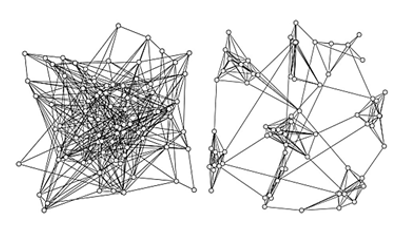
\includegraphics{https://raw.githubusercontent.com/Nertekkad/ml_nets/main/Images/Fig1.PNG}
\caption{\textbf{Figura 1:} Las redes generadas aleatoriamente (izquierda) tienden a tener un coeficiente de clusterización significativamente menor al de las llamadas redes de mundo pequeño (derecha), con el mismo número de nodos. Las redes de mundo pequeño se caracterizan por tener conjuntos de nodos estrechamente interconectados, a pesar de que la mayoría de sus elementos no sean vecinos entre sí. Imagen extraída de Schaeffer, 2007 \citep{schaeffer2007graph}.}
\end{figure}

El coeficiente de clusterización es una propiedad local, es decir, para cada nodo se define un valor de dicho coeficiente. Para determinar un valor global del coeficiente de clusterización de la red en su conjunto es simplemente el promedio aritmético de todos los coeficientes de clusterización.

\[C_{net}=\frac{1}{N}\sum_{i=1}^{N} C_{i}\]
Al tipo de redes donde la mayoría de los nodos no son vecinos entre sí se les conoce como redes de mundo pequeño. Los primeros en idear este coeficiente fueron Watts y Strogatz en 1988, y es gracias a esta propiedad que es posible diferenciar una red aleatoria de una red de mundo pequeño \citep{watts1998collective}.

\begin{figure}
\centering
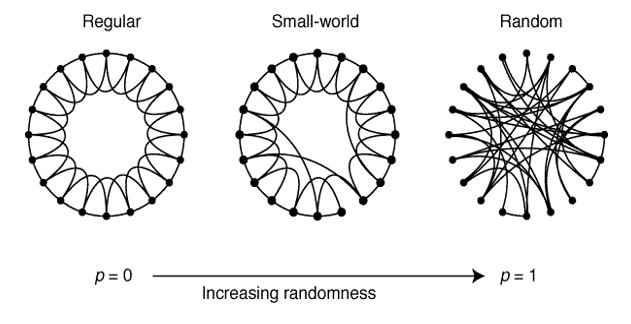
\includegraphics{https://raw.githubusercontent.com/Nertekkad/ml_nets/main/Images/Fig2.PNG}
\caption{\textbf{Figura 2:} La aleatoriedad de una red (\(p\)) es un factor importante en su arquitectura. Cuando este valor es igual a cero, los nodos poseerán exactamente el mismo número de conexiones y, por lo tanto, la distribución de su \emph{degree} será uniforme. Por el contrario, cuando los valores de aleatoriedad son cercanos a uno, dicha distribución se asemeja a una curva gaussiana, donde existirán nodos que posean muchas conexiones en un extremo de la distribución, otros con un número bajo de conexiones y la mayoría con un número de conexiones cercano a la media de la red.Imagen extraída de Watts y Strogatz, 1998 \citep{watts1998collective}.}
\end{figure}

\begin{figure}
\centering
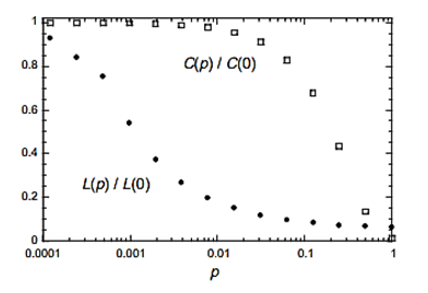
\includegraphics{https://raw.githubusercontent.com/Nertekkad/ml_nets/main/Images/Fig3.PNG}
\caption{\textbf{Figura 3:} Conforme aumenta la aleatoriedad de una red, el coeficiente de clusterización (\(C(p)\)) adquiere valores cada vez menores; al tiempo que la longitud de la red (\(L(p)\)), es decir, la distancia (cuantificada en número de aristas) más corta entre todos los posibles pares de nodos de una red, también disminuye. Imagen extraída de Watts y Strogatz, 1998 \citep{watts1998collective}.}
\end{figure}

Esta característica le brinda a la red robustez, es decir, la capacidad de conservar su arquitectura ante ataques aleatorios \citep{newmanoxford}. En sistemas biológicos, como pueden ser cascadas de señalización, de suceder mutaciones aleatorias que puedan alterar el funcionamiento normal de alguna proteína involucrada en determinada ruta de señalización, es estadísticamente más probable que dicha mutación ocurra en un elemento de la red con bajo número de conexiones a que suceda en algún elemento central de la red, lo cual permite que la célula pueda continuar sus funciones biológicas con relativa normalidad \citep{das2020small}. En este tipo de redes unos pocos nodos poseen la mayor parte de las conexiones, mientras que la mayoría de los nodos poseen un bajo número de estas \citep{newmanoxford}.

\begin{figure}
\centering
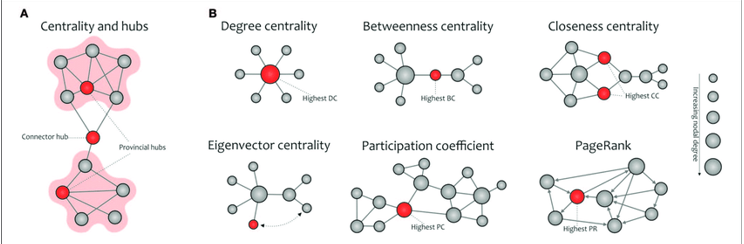
\includegraphics{https://raw.githubusercontent.com/Nertekkad/ml_nets/main/Images/Fig4.PNG}
\caption{\textbf{Figura 4:} La importancia de un nodo dentro de la red está determinada por su centralidad, misma que se puede determinar bajo distintos métodos. A) A aquellos nodos con una alta centralidad se les conoce como \emph{hubs} o conectores. B) La centralidad por \emph{degree} o grado se fundamenta en el número de conexiones de los nodos, mientras que la centralidad por intermediación o \emph{betweenness} otorga mayor peso a nodos que actúan como puentes entre clústers separados. La centralidad por \emph{closeness} o cercanía cuantifica el promedio de las distancias más cortas de cada nodo con todos los demás. La centralidad por eigenvectores, también conocida como \emph{eigencentrality}, es una medida autorreferencial de centralidad que prima la calidad de las conexiones, donde un nodo tendrá mayor relevancia si a su vez está conectado a un nodo con alta centralidad. El coeficiente de partición, por su parte, considera la distribución de las conexiones entre clústers separados. Finalmente, el \emph{PageRank} es una medida de centralidad similar al \emph{degree} pero empleada en redes dirigidas, y a menudo usada para determinar la importancia de páginas web. Imagen extraída de Farahani \emph{et al.}, 2019 \citep{farahani2019application}.}
\end{figure}

Sin embargo, los sistemas biológicos no suelen ser entes aislados, sino que se ven afectados por su interacción con aquello que los rodea. La idea de que los componentes de una red son capaces de interactuar o relacionarse de alguna forma con los elementos de otras redes, nos adentra en el concepto de las redes múltiples (\emph{multinetworks}), también conocidos como multigrafos (\emph{multigraphs}) o redes multicapa (\emph{multilayer networks}).

\hypertarget{definiciuxf3n-y-caracteruxedsticas-de-las-redes-multicapa}{%
\section*{Definición y características de las redes multicapa}\label{definiciuxf3n-y-caracteruxedsticas-de-las-redes-multicapa}}
\addcontentsline{toc}{section}{Definición y características de las redes multicapa}

Una red multicapa es una red compuesta por \(M\) redes individuales cuyos elementos interactúan entre sí, constituyendo cada una de estas redes individuales una capa \citep{buldyrev2010catastrophic}.

\[\cal{M}=\mathrm{(Y,\vec{G},\cal{G})}\]

Donde \(Y\) corresponde al conjunto de capas:

\[Y=\left \{ \alpha | \alpha \in \left \{ 1, 2, ... \space ,M \right \} \right \}\]

\(\vec{G}\) corresponde a la lista ordenada de redes que conforman cada una de las capas, donde cada elemento \(G_{\alpha}=(V_{\alpha}, E_{\alpha})\) es una red monocapa con sus propios nodos y aristas dentro de la red multicapa \citep{buldyrev2010catastrophic}.

\[\vec{G} = (G_{1}, G_{2}, ... \space , G_{\alpha }, ... \space , G_{M})\]

Por su parte, \(\cal{G}\) representa a una matriz \(MxM\) en la cual están contenidas las interacciones entre los nodos de cada par de redes que conforman la red multicapa. Debido a que en la matriz están representadas las interacciones entre cada par de redes, podemos entender el total como un conjunto de redes bipartitas \citep{buldyrev2010catastrophic}.

\[\cal{G} = (V_{\alpha},V_{\beta},\mathit{E_{\alpha, \beta}} )\]

Las redes multicapa se clasifican en tres categorías principales: las redes multiplex, redes temporales y redes formadas por redes \citep{bianconi2018multilayer}. Las redes multiplex son el ejemplo más sencillo de redes multicapa; estas se emplean generalmente cuando el mismo conjunto de nodos se encuentra contenido en las distintas capas, pero la interacción entre estos es distinta en cada una \citep{bianconi2018multilayer}. Las redes múltiplex son empleadas para mostrar cómo un mismo conjunto de elementos pueden interactuar entre sí de distintas formas, por lo general, asociando las aristas con un color distinto para cada tipo de interacción \citep{kanawati2015multiplex}. Por ejemplo, podríamos ejemplificar esto como un conjunto de individuos que se relacionan entre ellos por medio de distintas redes sociales \citep{aleta2019multilayer}. En biología, por ejemplo, podríamos construir una red multiplex donde una capa representa las correlaciones entre la expresión de distintos genes y otra capa representa las interacciones entre las proteínas que estos mismos genes codifican \citep{arda2019multiplex}.

Tomando como referente el último ejemplo, podemos también aludir al problema de los sistemas dinámicos. Los sistemas dinámicos son aquellos donde las interacciones cambian constantemente en función del tiempo, y, por lo tanto, la forma en que sus componentes están relacionados depende en gran medida del momento y las condiciones en las cuales se realiza la medición \citep{holme2012temporal}. Los sistemas biológicos son por lo general sistemas dinámicos, pues estos están constantemente sometidos a cambios debidos a estímulos con el ambiente que los rodea, así como a la naturaleza cambiante de los procesos que ocurren dentro de las células. Por ejemplo, un conjunto de genes no permanecerá siempre expresado de la misma manera, sino que la expresión de estos dependerá de un gran número de estímulos. Este tipo de sistemas se pueden representar mediante redes temporales, donde cada una de las capas representa una captura de las interacciones entre un conjunto de nodos en un momento determinado \citep{holme2012temporal}. Las redes temporales son secuenciales, es decir, que las capas están ordenadas de modo que se suceden una detrás de otra, por lo cual una capa \(t_{i}\) solo puede interactuar con la capa siguiente \(t_{i+1}\) \citep{barrat2008dynamical}. Este tipo de redes son similares a las redes multiplex en el sentido de que se trata del mismo conjunto de nodos entre las capas, aunque conforme avanza el tiempo nodos nuevos pueden integrarse a la capa siguiente mientras que otros dejan de estar presentes \citep{barrat2008dynamical}.

Finalmente podemos destacar las redes formadas por redes. Estas poseen importantes diferencias con respecto a los tipos de redes ya mencionados, empezando con que los nodos varían entre capa y capa; además de que los nodos de una capa no interactúan necesariamente solo con las capas adyacentes, como sí sucede con las redes multiplex o las redes temporales, sino que pueden interactuar con cualquier número de nodos en cualquiera de las capas \citep{kenett2015networks}.

\begin{figure}
\centering
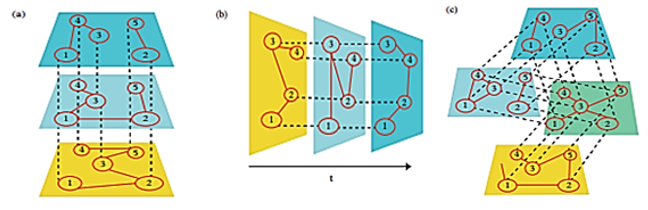
\includegraphics{https://raw.githubusercontent.com/Nertekkad/ml_nets/main/Images/Fig5.PNG}
\caption{\textbf{Figura 5:} Existen distintos tipos de redes multicapa, de las cuales podemos resaltar tres categorías. a) Las redes multiplex se caracterizan por mantener el mismo conjunto de nodos en sus distintas capas. Este tipo de redes suele emplearse para representar cómo los elementos de un conjunto interactúan entre sí de distintas formas o bajo distintas condiciones. b) Las redes temporales se usan para representar la forma en que un conjunto de elementos o nodos interactúa en función del tiempo. A diferencia de las redes multiplex, las capas de las redes temporales son secuenciales y se suceden de forma ordenada una tras otra, representando cada una las interacciones entre los distintos nodos a distintos ``momentos'' de un intervalo de tiempo definido. Estas son útiles para representar sistemas dinámicos, donde las interacciones entre sus componentes cambian continuamente. c) En las redes conformadas por redes, por su parte, las interacciones entre los elementos de una capa no están limitadas a las de las capas vecinas, sino que los nodos de cada capa pueden poseer un número de conexiones con los nodos de cualquiera de las capas de la red múltiple. Imagen extraída de Bianconi, 2018 \citep{bianconi2018multilayer}.}
\end{figure}

Debido a que las interacciones entre capas de una red multiplex están limitadas a las capas vecinas con respecto a la capa de referencia, podemos representar a una red múltiplex como una red bidimensional con conexiones de distintos tipos. En este tipo de redes los nodos de una capa solo se conectan con sus homólogos en la siguiente, además de que el conjunto de estos se mantiene en las distintas capas, variando solo las interacciones entre los nodos dentro de las mismas capas \citep{kanawati2015multiplex}.

\begin{figure}
\centering
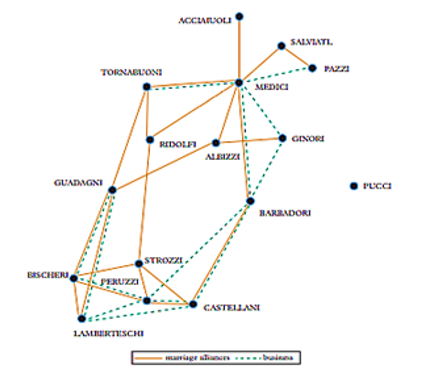
\includegraphics{https://raw.githubusercontent.com/Nertekkad/ml_nets/main/Images/Fig6.PNG}
\caption{\textbf{Figura 6:} Las redes multiplex muestran cómo los nodos de una red pueden interactuar entre sí de distintas formas. En este ejemplo se muestran los vínculos matrimoniales y de negocios entre distintas familias nobles florentinas del siglo XV. Utilizando esta representación, podemos vislumbrar con facilidad el papel central que tenía la familia Medici tanto en el ámbito comercial como político entre la nobleza florentina. Imagen extraída de Biaconti, 2018 \citep{padgett1993robust}.}
\end{figure}

\[\cal{M} = \mathit{(Y,\vec{G})}\]
Donde
\[\vec{G} = (G_{1}, G_{2}, ... \space ,G_{\alpha}, ... \space ,G_{M})\]

Cada una de las capas de la red multiplex poseen la misma cantidad de nodos
\[V = \left \{ i|i \in \left \{ 1,2,...,N \right \} \right \}\]

Sin embargo, a pesar de que las redes multiplex presentan el mismo grupo de nodos en las distintas capas, a menudo es necesario distinguir la capa en la cual se encuentra cada uno de los nodos \citep{bianconi2018multilayer}.
\[V = \left \{ i_\alpha |i \in \left \{ 1,2,...,N \right \} \right \}\]

Tanto para redes múltiplex como para redes temporales, la conexión de los nodos entre capa y capa está dada por la delta de Kronecker. Esta es una función cuya variable puede adquirir un valor de 1 en aquellos casos donde un elemento sea igual en dos conjuntos, o en este caso en dos capas, y de 0 cuando son diferentes. Aquellos nodos que cumplen la condición de ser equivalentes entre una capa y otra se denominan nodos réplica \citep{gomez2013diffusion}.

\[\delta _{ij} = \left\{\begin{matrix}
1 \space si  \space i=j \\ 
0 \space si  \space i\neq j
\end{matrix}\right.\]

Como hemos visto previamente, la información de una red simple está contenida dentro de una matriz de adyacencia, sin embargo, en redes multicapa este modelo resulta insuficiente para contener la información de estas estructuras, razón por la cual empleamos las llamadas matrices de supra-adyacencia. Este tipo de matrices están compuestas a partir de múltiples matrices de adyacencia individuales, y contiene tanto la información referente a las interacciones dentro de las capas como las interacciones entre capas \citep{cozzo2016multilayer}.

\begin{figure}
\centering
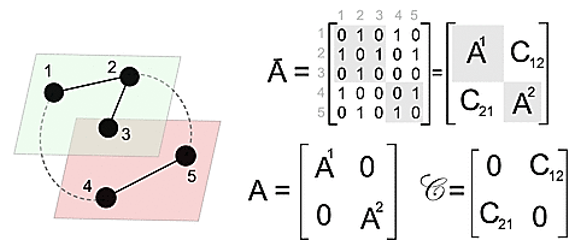
\includegraphics{https://raw.githubusercontent.com/Nertekkad/ml_nets/main/Images/Fig7.PNG}
\caption{\textbf{Figura 7:} A la derecha se muestra la representación tridimensional de una red bipartita. La matriz de supra-adyacencia (\(\bar{A}\)) está compuesta a partir de la fusión de dos matrices de adyacencia simples. La primera es la matriz \(A\), que codifica las interacciones de los nodos dentro de las capas, mientras que la matriz \(C\) contiene las interacciones entre las capas. Imagen extraída de Cozzo \emph{et al.}, 2016 \citep{cozzo2016multilayer}.}
\end{figure}

Como se puede inferir, las propiedades de las redes múltiples difieren de las redes simples. Como ya hemos visto, el \emph{degree} (\(k_{i}\)) de un nodo de una red simple es un escalar, un número entero positivo que representa el número de conexiones de un nodo. En redes múltiples este valor está representado en un vector M-dimensional que contiene los valores del \emph{degree} de un nodo ``\(i\)'' a lo largo de las \(M\) capas de la red \citep{iacovacci2016functional}.

\[k_{i} = (k_{i}^{[1]}, k_{i}^{[2]},..., k_{i}^{[M]})\]
Al igual que como sucede con redes simples, la distribución del \emph{degree} es una función de probabilidad \(P^{[a]}(k)\). En redes múltiples, esta función de probabilidad se define de forma independiente para cada capa \citep{iacovacci2016functional}.

\[P^{[a]}(k) = \frac{N^{[a]}(k)}{N_{a}}\]
El coeficiente de clusterización en una red multiplex, al igual que sucede con las redes simples, permite conocer si existen conjuntos donde varios nodos están interconectados entre sí, sólo que, en este caso, esto también incluye las conexiones que se generan entre las capas \citep{lancichinetti2012consensus}. En redes sociales, por ejemplo, esta propiedad permitirá conocer la probabilidad de que dos individuos realicen varias actividades juntos, o que dos personas en dos clases distintas tengan algún amigo en común \citep{bianconi2018multilayer}. En biología, por ejemplo, el coeficiente de clusterización podría emplearse para saber si dos genes que se sobreexpresan en distintos pacientes analizados, podrían estar involucrados en el mismo proceso \citep{zuzek2015epidemic}. El problema de la clusterización en redes múltiples es que los ciclos de longitud, los mismos que generan triángulos de nodos interconectados en redes simples, se completan en capas distintas, lo que complica su identificación \citep{lancichinetti2012consensus}.

\begin{figure}
\centering
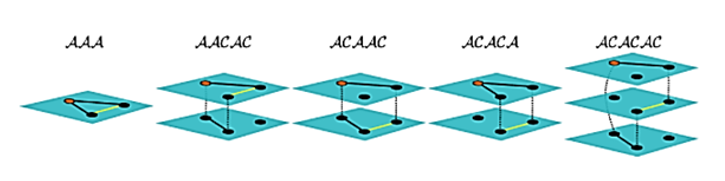
\includegraphics{https://raw.githubusercontent.com/Nertekkad/ml_nets/main/Images/Fig8.PNG}
\caption{\textbf{Figura 8:} En el extremo izquierdo de la imagen se muestra una red simple donde los dos vecinos del nodo \(i\) (marcado en rojo), están conectados entre sí. En los siguientes tres diagramas se muestran ejemplos de redes bipartitas donde, con respecto a la capa donde se encuentra el nodo \(i\), un grupo de nodos pueden no ser vecinos en dicha capa, pero si en una capa distinta, permitiendo la formación de ciclos entre ambas capas. En el extremo derecho de la imagen podemos ver un ejemplo en el cual se ejemplifica cómo estos ciclos de nodos interconectados no necesariamente se limitan a dos capas, sino que pueden extenderse a más capas. Imagen extraída de Cozzo \emph{et al.}, 2013 \citep{cozzo2013clustering}.}
\end{figure}

De forma similar a como hemos visto en redes simples, podemos obtener este coeficiente dividiendo el número de triángulos que se forman entre los nodos de distintas capas sobre el producto del número de vecinos (\emph{degree}) de la primera y última capa (\(N_{\alpha, \gamma}\)) \citep{cozzo2013clustering}.

\[C_{i}^{[\alpha,\beta,\gamma]}=\frac{\sum_{r,s}a^{[\alpha]}_{ir}a^{[\beta]}_{rs}a^{[\gamma]}_{si}}{N_{\alpha, \gamma}}\]

Donde:

\[N_{\alpha, \gamma} = \left\{\begin{matrix}
k^{[\alpha]}_{i}k^{[\gamma]}_{i} \space para \space  \alpha \neq \gamma \\
k^{[\alpha]}_{i}(k^{[\alpha]}_{i}-1) \space para \space  \alpha = \gamma
\end{matrix}\right. \]

Así como sucede en lo referente a la transitividad, la cuantificación de otras propiedades de la red, tales como las distancias entre los nodos, difieren cuando tratamos con redes multicapa. Inferir la distancia más corta entre cualquier par de nodos implica ahora considerar las distancias entre capas \((\psi_{ij})\), además de las distancias más cortas dentro de la misma capa \((\sigma_{ij})\). La fracción resultante nos permite conocer la accesibilidad entre los nodos, una propiedad a la cual denominamos interdependencia (\(\lambda_{i}\)), cuyo valor fluctúa entre 1 y 0 \citep{donges2011investigating}.

\[\lambda_{i} = \sum_{i \neq j}\frac{\psi_{ij}}{\sigma_{ij}}\]

La interdependencia media de la red multicapa puede expresarse como:

\[\lambda = \frac{1}{N}\sum_{i=1}^{N}\lambda_{i}\]

Cuando \(\lambda\) posee un valor equivalente o muy cercano a 0, significa que existe una muy baja interdependencia entre las capas, ya que todas o la gran mayoría de las rutas más cortas entre cualquier par de nodos se encuentran dentro de la misma capa. Lo contrario sucede cuando \(\lambda\) adquiere valores cercanos o equivalentes a 1, la interdependencia de los nodos entre las capas es muy alta \citep{donges2011investigating}.

El análisis de las propiedades de la red puede arrojar indicios sobre el comportamiento del sistema en su conjunto, así como información que ayude a explicar ciertos fenómenos que ocurren cuando estudiamos ejemplos reales de sistemas complejos.

\hypertarget{aplicaciones-de-las-redes-multicapa}{%
\section*{Aplicaciones de las redes multicapa}\label{aplicaciones-de-las-redes-multicapa}}
\addcontentsline{toc}{section}{Aplicaciones de las redes multicapa}

Las redes multicapa representan un enfoque relativamente nuevo en teoría de redes y en el análisis de sistemas complejos. Los sistemas complejos son aquellos que están compuestos por un número muy grande de distintos elementos que interactúan, de forma no lineal, entre sí \citep{liu2016control}. A medida que el estudio de este tipo de sistemas avanzaba, fue evidente pronto que no se trataba de sistemas aislados, y que, por el contrario, se requería de una nueva perspectiva que ampliara nuestra capacidad para analizarlos, dando lugar al enfoque de las redes multicapa \citep{bianconi2018multilayer}. Las redes multicapa son ubicuas, podemos encontrar ejemplos en casi todo aquello que nos rodea; desde la evolución de las conexiones neuronales con respecto al tiempo, las interacciones entre el proteoma, el genoma y el transcriptoma, hasta el internet, los medios de transporte urbano en una ciudad o las interacciones entre las distintas partículas elementales \citep{bianconi2018multilayer}.

\begin{figure}
\centering
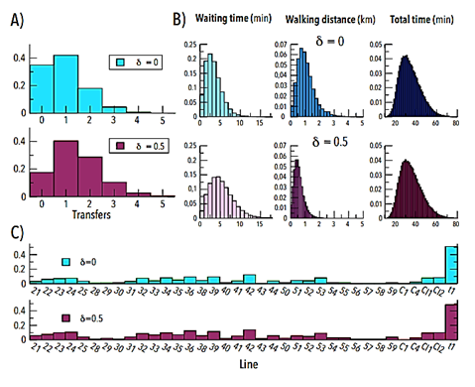
\includegraphics{https://raw.githubusercontent.com/Nertekkad/ml_nets/main/Images/Fig9.PNG}
\caption{\textbf{Figura 9:} Mediante el análisis de las propiedades de las redes múltiples a gran escala es posible obtener información sobre el comportamiento de un sistema. En el ejemplo se realizó la simulación de un modelo basado en el sistema de transporte de Zaragoza, España. a) Distribución del número de veces que los individuos pudieron llegar a su destino en el intervalo de tiempo en que se realizó la simulación. b) Distribución del tiempo de espera, la distancia recorrida y la duración del recorrido empleando dos velocidades de movimiento distintas (\(\delta\)). c) Fracción de pasajeros que usaron las distintas líneas de transporte. Este tipo de simulaciones se ha empleado para buscar alternativas que permitan mejorar la eficiencia de un sistema de transporte público.Imagen extraída de Aleta \emph{et al.}, 2017 \citep{aleta2017multilayer}.}
\end{figure}

En sistemas complejos, estas interacciones dan lugar a propiedades emergentes, cualidades o características sólo discernibles a macroescala pero que no pueden ser predichas únicamente mediante el estudio de las partes constituyentes de la red, patrones que sólo pueden conocerse cuando se observa el resultado de la interacción de sus partes constituyentes. Los ejemplos de propiedades emergentes son variados, tales como la conciencia o la inteligencia, producto de las billones de interacciones entre neuronas \citep{o1994emergent} nuestras sociedades, en donde la formación de naciones puede considerarse como una propiedad emergente de la interacción humana \citep{lazega1999multiplexity}; los organismos como producto de la interacción entre millones de células; o los organismos mismos como parte de un ecosistema \citep{liu2016control}. En cualquiera de estos casos, el estudio de una sola neurona como unidad no permitiría comprender a la conciencia humana, así como el estudio de un solo individuo no permitiría predecir el comportamiento de una civilización, o el de una célula el comportamiento de todo un organismo vivo formado por millones de estas. En cualquier caso, la comprensión de un sistema complejo requiere el análisis de su estructura y comportamiento en su conjunto, sin embargo, la interacción de los elementos de una red no se limita necesariamente a los elementos dentro de la red, una idea que posteriormente dio paso al concepto de redes multicapa \citep{bianconi2018multilayer}.

Aunque las redes multicapa se estudiaron originalmente en el contexto de las ciencias sociales con el fin de representar la forma en que distintas personas establecen lazos de formas diferentes, por ejemplo, a través de las relaciones laborales, de amistad o mediante distintas redes sociales \citep{lazega1999multiplexity}; el uso de este enfoque se ha extendido a muchos otros campos, y las ciencias biológicas no han sido la excepción. Desde la neurociencia y la biología molecular hasta la ecología y la epidemiología, las redes multicapa han tenido multitud de aplicaciones dentro del campo de la biología y la medicina.

\begin{figure}
\centering
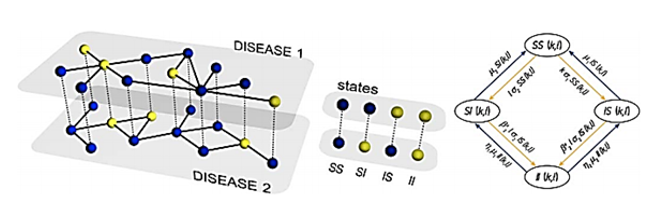
\includegraphics{https://raw.githubusercontent.com/Nertekkad/ml_nets/main/Images/Fig10.PNG}
\caption{\textbf{Figura 10:} Una de las aplicaciones más recurrentes en biología de las redes multicapa es en el campo de la epidemiología, en donde se aplican redes temporales para predecir el comportamiento de un brote infeccioso en una población. En el ejemplo se muestra una representación de un modelo susceptible-infectado-susceptible (SIS), donde la interacción entre los individuos propicia que un nodo cambie su estado como susceptible a infectados o nuevamente susceptibles en la siguiente capa, dependiendo de su estado anterior. Además, en este tipo de modelos los individuos cambian su interacción en el tiempo, y la probabilidad de que un individuo pase de un estado al otro depende de una determinada tasa de cambio. Imagen extraída de Sanz \emph{et al.}, 2014 \citep{sanz2014dynamics}.}
\end{figure}

Podemos aludir al ejemplo de las redes entre genes, mismas que a su vez producen proteínas cuya interacción genera un efecto en las células, a la vez que regulan el sistema a distintos niveles. (genoma, epigenoma, transcriptoma, proteoma y metaboloma). A este conjunto de biomoléculas en interacción que constituyen una célula es a lo que llamamos interactoma \citep{aleta2019multilayer}. Una proteína producida por determinado gen puede regular positiva o negativamente a otro gen al realizar una modificación epigenética sobre este, así como un siRNA es capaz de regular la traducción a proteína de determinado transcrito. Como podemos ver con este ejemplo, la regulación de la red puede ocurrir a distintos niveles y mediante la interacción de elementos de alguna capa con cualquiera de las otras capas \citep{sun2016integrative}.

\begin{figure}
\centering
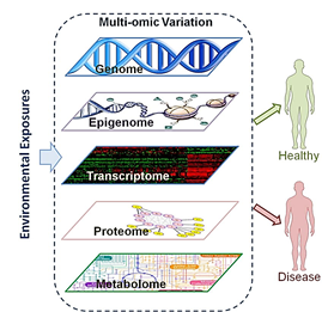
\includegraphics{https://raw.githubusercontent.com/Nertekkad/ml_nets/main/Images/Fig11.PNG}
\caption{\textbf{Figura 11:} La regulación de las respuestas celulares a los estímulos ambientales puede darse a distintos niveles, desde la expresión de génica, la traducción de transcritos o la actividad de las proteínas. Las alteraciones en los mecanismos de regulación del organismo se han asociado a múltiples enfermedades, y nos han permitido profundizar nuestro conocimiento al respecto de estas. Imagen extraída de Sun y Hu, 2016 \citep{sun2016integrative}.}
\end{figure}

El análisis del interactoma mediante redes multicapa también ha sido útil para comprender los efectos de fármacos en los complejos procesos que ocurren dentro de una célula, pues integra los distintos niveles de regulación celular y la forma en que estos se ven alterados en respuesta a determinado medicamento \citep{aleta2019multilayer}. De igual modo, ciertos patrones de expresión génica anormales se han asociado a distintos tipos de cáncer o a enfermedades crónico-degenerativas \citep{albert2002statistical}.

El mapeo de redes cerebrales mediante redes temporales ha adquirido gran importancia también. Las redes multicapa permiten representar detalladamente las interacciones sinápticas entre neuronas y su evolución ante estímulos. La gran mayoría de los estudios al respecto se han centrado en \emph{C. elegans}, un nemátodo que ofrece numerosas facilidades al momento de estudiar su sistema nervioso, pues además de ser un modelo de estudio ampliamente conocido, también posee un número reducido y limitado de neuronas. Se han empleado redes múltiples para analizar la señalización aminérgica y neuro peptídica entre las 302 neuronas de \emph{C. elegans}, asociando una capa distinta para cada neurotransmisor involucrado en la comunicación sináptica \citep{bentley2016multilayer}. En humanos el enfoque de las redes múltiples se ha empleado para estudiar las relaciones entre distintas zonas del cerebro y las respuestas cerebrales en reposo mediante procedimientos no invasivos, tales como la resonancia magnética \citep{del2016synchronization}.

En ecología, el enfoque de las redes multicapa ha sido de suma utilidad para comprender las interacciones entre los distintos organismos que componen un ecosistema. La construcción de redes tróficas no solo ha permitido comprender mejor el flujo de materia y energía dentro de un ecosistema, sino también la importancia de las relaciones simbióticas y cómo estas afectan la estabilidad del ecosistema y las poblaciones, por ejemplo, la relación entre las plantas angiospermas y los insectos polinizadores \citep{schleuning2020trait}. Dentro de las redes tróficas se consideran distintos factores, incluyendo el peso o fuerza de la interacción y el tipo de esta (mutualismo, amensalismo, parasitismo, comensalismo, depredación, etc.), pudiendo representar los distintos tipos de interacción en una red tipo multiplex \citep{schweiger2008climate}.

El análisis mediante redes temporales ha arrojado información sobre el cambio de las interacciones entre organismos en respuesta al cambio climático, a la deforestación o a la contaminación. La reducción de la biodiversidad debida directa o indirectamente a la actividad humana altera la estructura de la red, provocando también cambios en poblaciones de organismos relacionados con aquellos cuyas poblaciones se han alterado debido a la actividad humana \citep{schweiger2008climate}. Se ha observado que la extinción de ciertas especies ha provocado también la caída de las poblaciones de otras especies relacionadas con las primeras, o, por el contrario, sus poblaciones aumentan exponencialmente, derivando en el fenómeno de las plagas \citep{ludwig1978qualitative}. También se han empleado redes temporales para estudiar el comportamiento de animales sociales, tales como hormigas, y la forma en que estos lazos sociales ayudan al éxito de las comunidades en general \citep{schleuning2020trait}.

\begin{figure}
\centering
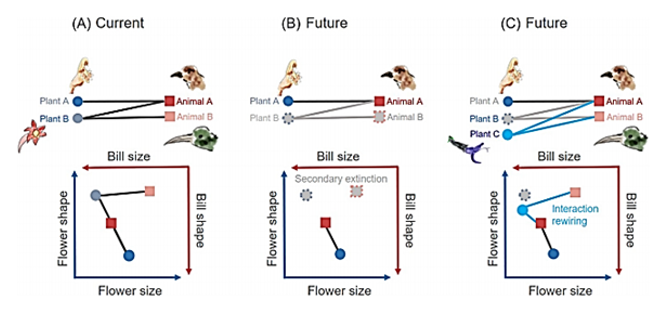
\includegraphics{https://raw.githubusercontent.com/Nertekkad/ml_nets/main/Images/Fig12.PNG}
\caption{\textbf{Figura 12:} En un ecosistema se dan múltiples interacciones entre distintos organismos. La estabilidad del ecosistema en sí mismo, depende en gran medida de estas interacciones, pues la extinción de una especie puede conllevar a extinciones secundarias de especies que, en mayor o menor medida, dependían de las poblaciones de la primera especie. En el ejemplo se muestran plantas con flores que dependen de aves como polinizadoras y viceversa. Algunas especies con relaciones mutualistas han evolucionado para adaptar sus características para facilitar la interacción entre ellas, en este caso la forma de las flores o del pico en sus respectivos casos; sin embargo, esto provoca que ambas especies sean más interdependientes entre sí, y, por lo tanto, más proclives a extinguirse en el caso de que la población de cualquiera de las dos especies entre en declive o se extinga. En ocasiones, la entrada de alguna especie exógena al ecosistema puede suplir la función de la especie extinta y favorecer la recuperación de las poblaciones de su simbionte, sin embargo, con frecuencia la introducción de nuevas especies puede tener un efecto contrario al provocar el desplazamiento por competencia de las especies nativas. Imagen extraída de Schleuning \emph{et al.}, 2020 \citep{schleuning2020trait}.}
\end{figure}

\hypertarget{inferencias-de-redes}{%
\section*{Inferencias de redes}\label{inferencias-de-redes}}
\addcontentsline{toc}{section}{Inferencias de redes}

Hemos visto que la creación de redes temporales y redes multiplex es posible mediante la delta de Kronecker, dicha función permite conectar los nodos de una capa con sus respectivos nodos réplica en las capas adyacentes. Sin embargo, al intentar construir las redes de cada capa nos encontramos con un problema: Construir una red a partir de los datos experimentales. Como solución se han propuesto numerosos algoritmos que llevan a cabo la tarea de inferir las posibles asociaciones entre los componentes de una red partiendo de las abundancias de secuencias en las muestras, mismas que pueden asociarse a OTUs o transcritos de genes.

Para identificar la presencia de algún microorganismo o la expresión de algún gen a partir de una muestra se emplean métodos de amplificación de ácidos nucleicos, tales como el PCR o el RT-PCR, con el fin de identificar secuencias específicas. A partir del análisis de estas secuencias se obtienen las abundancias relativas, mismas que pueden interpretarse como el volumen de las secuencias identificadas en una muestra \citep{villaintroduction}.

Podemos organizar los datos dentro de una matriz \(n x p\) , donde \(n\) representa el conjunto de muestras y \(p\) la lista de secuencias identificadas, siendo por lo general \(n<p\). Cada elemento de la matriz representa la abundancia de una secuencia \(j\) en una muestra \(i\). A partir de esta información podemos construir una matriz de similaridad, misma que representan las similaridades entre las abundancias relativas entre las secuencias. Con base en dicha matriz, podemos conectar aquellas secuencias identificadas o nodos (OTUs, genes, transcritos, etc.) que posean una mayor correlación entre ellas \citep{butte1999unsupervised}. Existen numerosos algoritmos capaces de realizar esta tarea, mismos que analizaremos a continuación.

La forma más sencilla de generar una red a partir de una matriz de similaridad es eliminando todos aquellos elementos de la matriz cuya similitud sea demasiado débil, es decir, que se encuentre por debajo de determinado umbral \citep{villaintroduction}. A partir de la matriz resultante se genera una matriz de adyacencia, donde todos aquellos valores por encima del umbral seleccionado son considerados como conexiones entre las secuencias asociadas a algún gen o microorganismo específico, mismos que representamos como nodos dentro de la red \citep{butte1999mutual}.

\begin{figure}
\centering
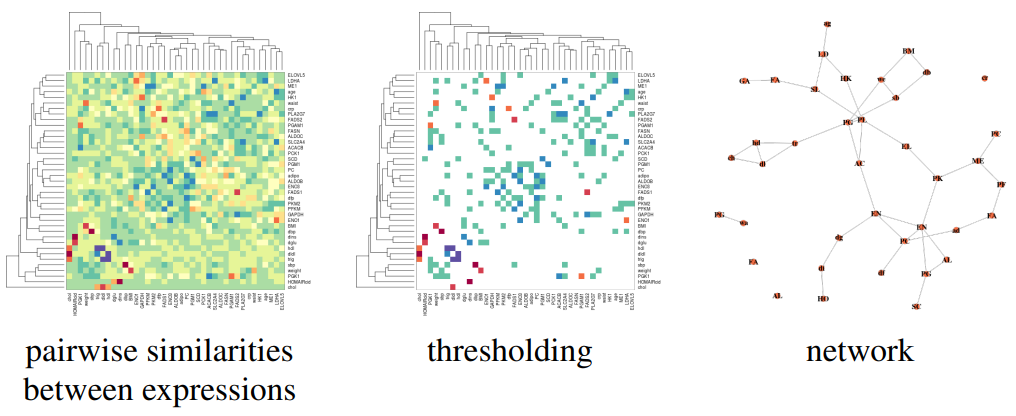
\includegraphics{https://raw.githubusercontent.com/Nertekkad/ml_nets/main/Images/Fig13.PNG}
\caption{\textbf{Figura 13:} El principio básico de un algoritmo de inferencia de redes es la generación de una matriz de similaridad que represente las relaciones de co-abundancia de las secuencias identificadas a partir de los datos muestrales. Cada una de las distintas secuencias encontradas serán consideradas como nodos de la futura red. Todos los valores de la matriz de similaridad que se encuentren por debajo del umbral establecido por el investigador, son descartados. A partir de los valores restantes se genera una matriz de adyacencia a partir de la cual se construye una red. Imagen extraída de Villa-Vialaneix-nathalie \citep{villaintroduction}.}
\end{figure}

Un ejemplo de este método de inferencia es el algoritmo del paquete WGCNA (\emph{Weighted Gene Correlation Network Analysis}) de R, empleado en el análisis de correlaciones en redes pesadas \citep{butte1999mutual}. El algoritmo fue diseñado para el análisis de co-expresión de genes, permitiendo hallar módulos o clústeres de genes con expresión génica similar, mismos que en teoría podrían estar implicados en las mismas rutas metabólicas o rutas de señalización; esto bajo la premisa de que los genes suelen expresarse (transcribirse y traducirse) de forma coordinada y en proporciones similares cuando determinado proceso celular está sucediendo, potencialmente estarían involucrados en dicho proceso \citep{langfelder2008wgcna}.

El algoritmo WGCNA procesa las co-abundancias de los transcritos, expresadas en un \emph{heatmap} como el peso asociado a las aristas, en un dendrograma o árbol. Esto permite clusterizar conjuntos de genes con una expresión similar entre las muestras a partir de las ramas principales del dendrograma \citep{zhang2005general}.

\begin{figure}
\centering
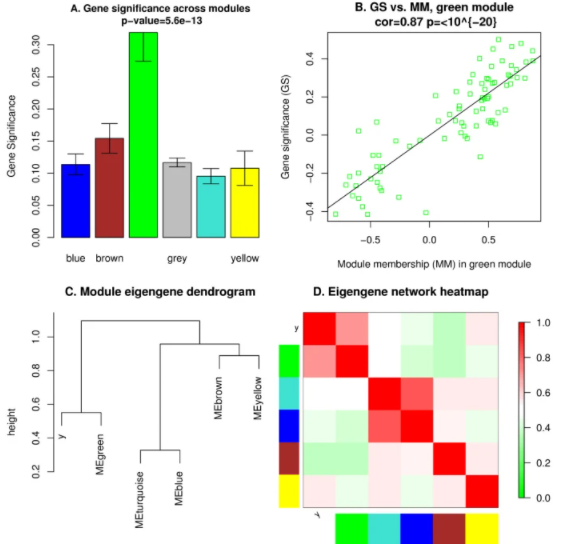
\includegraphics{https://raw.githubusercontent.com/Nertekkad/ml_nets/main/Images/Fig14.PNG}
\caption{\textbf{Figura 14:} El algoritmo WGCNA construye los módulos a partir de las abundancias de los transcritos en las muestras. Esto permite calcular la significancia media de cada módulo en conjunto con metadatos (como podrían ser categorías GO, que relacionan los genes con alguna característica o rasgo común y relacionar cada módulo con características clínicas). Entre mayor sea la significancia de un módulo mayor será la probabilidad de que dichos genes, representados en la red como nodos, estén relacionados. El dendrograma permite visualizar el agrupamiento jerárquico de estos genes en torno a las ramificaciones principales. Imagen extraída de Langfelder y Horvath, 2008 \citep{langfelder2008wgcna}.}
\end{figure}

Sin embargo, el hecho de que dos elementos de la matriz de similaridad posean una correlación alta no implica necesariamente que ambos estén directamente relacionados. Esto implica que el método anteriormente mencionado puede llevar a falsas interpretaciones en cuanto a cómo los nodos están conectados entre sí \citep{butte1999mutual}. Por ejemplo, si tenemos tres genes codificantes para tres productos (\(a\), \(b\) y \(c\)) que hemos analizado a lo largo de un centenar de muestras, y suponemos que el producto de \(a\) regula directamente a \(b\) y a \(c\), esperamos que exista una fuerte correlación entre la expresión de estos genes \citep{villaintroduction}. Sin embargo, cuando calculamos la correlación entre los genes \(b\) y \(c\), obtenemos un resultado muy parecido al de los casos anteriores, teniendo estos una correlación fuerte a pesar de no estar directamente vinculados, pero sí relacionados indirectamente mediante su mutua regulación a través del producto del gen \(a\).

\begin{Shaded}
\begin{Highlighting}[]
\KeywordTok{library}\NormalTok{(igraph)}
\end{Highlighting}
\end{Shaded}

\begin{verbatim}
## 
## Attaching package: 'igraph'
\end{verbatim}

\begin{verbatim}
## The following objects are masked from 'package:stats':
## 
##     decompose, spectrum
\end{verbatim}

\begin{verbatim}
## The following object is masked from 'package:base':
## 
##     union
\end{verbatim}

\begin{Shaded}
\begin{Highlighting}[]
\CommentTok{#Gráfico de ejemplo}
\NormalTok{gA <-}\StringTok{ }\KeywordTok{graph}\NormalTok{(}\KeywordTok{c}\NormalTok{(}\StringTok{"a"}\NormalTok{, }\StringTok{"b"}\NormalTok{, }\StringTok{"a"}\NormalTok{, }\StringTok{"c"}\NormalTok{))}
\KeywordTok{plot}\NormalTok{(gA, }\DataTypeTok{vertex.color=}\KeywordTok{c}\NormalTok{( }\StringTok{"red"}\NormalTok{, }\StringTok{"green"}\NormalTok{, }\StringTok{"yellow"}\NormalTok{))}
\end{Highlighting}
\end{Shaded}

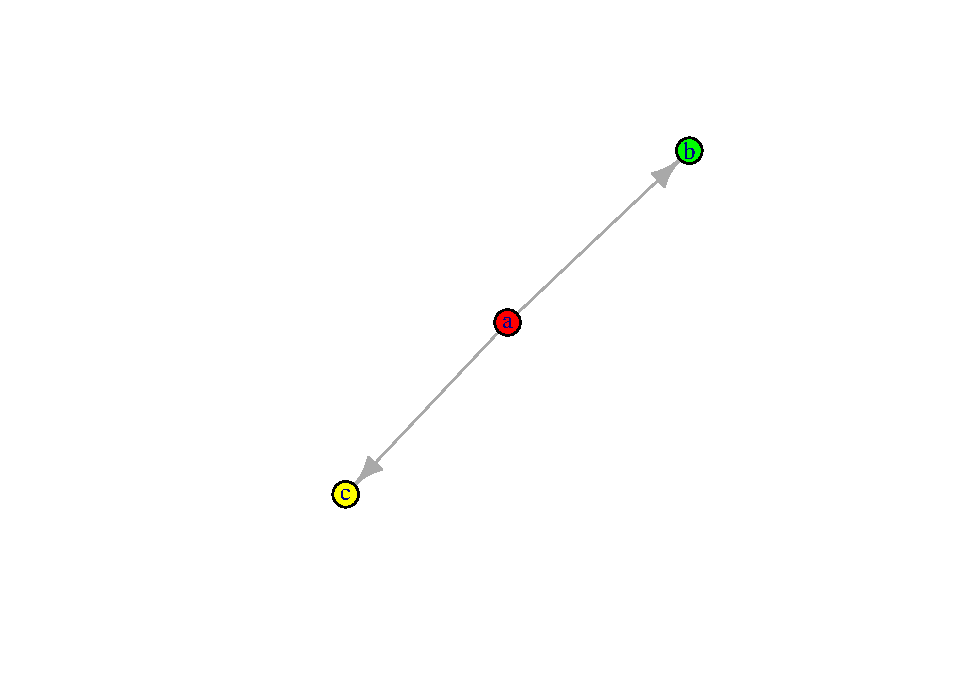
\includegraphics{_main_files/figure-latex/unnamed-chunk-1-1.pdf}

\begin{Shaded}
\begin{Highlighting}[]
\CommentTok{#Generamos un set de datos de prueba y calculamos la correlación entre los nodos.}
\KeywordTok{set.seed}\NormalTok{(}\DecValTok{2812}\NormalTok{)}
\NormalTok{a <-}\StringTok{ }\KeywordTok{rnorm}\NormalTok{(}\DecValTok{100}\NormalTok{, }\DecValTok{0}\NormalTok{, }\FloatTok{0.1}\NormalTok{)}
\NormalTok{b <-}\StringTok{ }\DecValTok{2}\OperatorTok{*}\NormalTok{a}\DecValTok{-2}\OperatorTok{+}\KeywordTok{rnorm}\NormalTok{(}\DecValTok{100}\NormalTok{,}\DecValTok{0}\NormalTok{,}\FloatTok{0.1}\NormalTok{)}
\KeywordTok{cor}\NormalTok{(a,b)}
\end{Highlighting}
\end{Shaded}

\begin{verbatim}
## [1] 0.9047034
\end{verbatim}

\begin{Shaded}
\begin{Highlighting}[]
\NormalTok{c <-}\StringTok{ }\DecValTok{2}\OperatorTok{*}\NormalTok{a}\OperatorTok{+}\DecValTok{4}\OperatorTok{+}\KeywordTok{rnorm}\NormalTok{(}\DecValTok{100}\NormalTok{,}\DecValTok{0}\NormalTok{,}\FloatTok{0.1}\NormalTok{)}
\KeywordTok{cor}\NormalTok{(a,c)}
\end{Highlighting}
\end{Shaded}

\begin{verbatim}
## [1] 0.9056657
\end{verbatim}

\begin{Shaded}
\begin{Highlighting}[]
\KeywordTok{cor}\NormalTok{(c,b)}
\end{Highlighting}
\end{Shaded}

\begin{verbatim}
## [1] 0.7763894
\end{verbatim}

\begin{figure}
\centering
\includegraphics{https://raw.githubusercontent.com/Nertekkad/ml_nets/main/Images/Fig15.PNG}
\caption{\textbf{Figura 15:} Como podemos observar en el ejemplo, el producto del gen \(a\) regula directamente a los productos de los genes \(b\) y \(c\), sin embargo, esto también provoca que exista una fuerte correlación entre los genes \(b\) y \(c\) a pesar de que la relación entre ambos sea en realidad indirecta.}
\end{figure}

Claramente, este tipo de correlaciones indirectas puede llevar a interpretaciones erróneas de los datos experimentales, por lo cual es necesario disponer de métodos que permitan descartar este tipo de falsos positivos. Bajo esta perspectiva, los modelos gráficos gaussianos\citep{uhler2017gaussian}, empleados para modelar las relaciones estadísticas entre variables de interés, son una herramienta útil para identificar y descartar interacciones indirectas gracias a que permiten estimar la dependencia condicional entre los nodos \citep{villaintroduction}.

En el siguiente ejemplo, basado en la simulación realizada previamente, podemos observar, además de que las correlaciones tienden a ser menos fuertes que en el primer modelo, que la correlación entre \(b\) y \(c\) posee valores negativos o significativamente más pequeños con respecto a los valores obtenidos para las correlaciones entre \(a\) y los nodos \(b\) y \(c\). El modelo calcula las correlaciones parciales, es decir, la correlación entre los residuos de los modelos lineales generados a partir de las variables \citep{villaintroduction}.

\begin{Shaded}
\begin{Highlighting}[]
\CommentTok{#Correlaciones mediante un modelo lineal}
\KeywordTok{cor}\NormalTok{(}\KeywordTok{lm}\NormalTok{(a}\OperatorTok{~}\NormalTok{c)}\OperatorTok{$}\NormalTok{residuals,}\KeywordTok{lm}\NormalTok{(b}\OperatorTok{~}\NormalTok{c)}\OperatorTok{$}\NormalTok{residuals)}
\end{Highlighting}
\end{Shaded}

\begin{verbatim}
## [1] 0.7542552
\end{verbatim}

\begin{Shaded}
\begin{Highlighting}[]
\KeywordTok{cor}\NormalTok{(}\KeywordTok{lm}\NormalTok{(a}\OperatorTok{~}\NormalTok{b)}\OperatorTok{$}\NormalTok{residuals,}\KeywordTok{lm}\NormalTok{(c}\OperatorTok{~}\NormalTok{b)}\OperatorTok{$}\NormalTok{residuals)}
\end{Highlighting}
\end{Shaded}

\begin{verbatim}
## [1] 0.756993
\end{verbatim}

\begin{Shaded}
\begin{Highlighting}[]
\KeywordTok{cor}\NormalTok{(}\KeywordTok{lm}\NormalTok{(b}\OperatorTok{~}\NormalTok{a)}\OperatorTok{$}\NormalTok{residuals,}\KeywordTok{lm}\NormalTok{(c}\OperatorTok{~}\NormalTok{a)}\OperatorTok{$}\NormalTok{residuals)}
\end{Highlighting}
\end{Shaded}

\begin{verbatim}
## [1] -0.2378752
\end{verbatim}

Es a partir de este principio que actúan algoritmos de inferencia de redes tales como ARACNE, CLR y MRNET, mismos que podemos encontrar en el paquete \emph{minet} de R. Estos algoritmos, además, se combinan con estimadores de entropía con el fin de corregir los sesgos asociados al ruido y ajustar la varianza de los datos \citep{villaintroduction}. Las redes generadas a partir de ellos se conocen como redes de información mutua, pues que son el resultado de la inferencia de conexiones entre pares de nodos con de puntuaciones altas de información mutua; refiriéndose la correlación fuerte entre dos variables a partir de modelos de dependencia no-lineal, que con frecuencia se ajustan mejor a las nubes de datos de las variables que los modelos lineales. Por consiguiente, los algoritmos premian las interacciones directas sobre las indirectas, otorgando valores bajos a las correlaciones entre nodos no relacionados directamente \citep{meyer2008minet}.

El algoritmo CLR es una extensión del modelo clásico de redes de relevancia, pues calcula una puntuación empírica asociada a los valores de la matriz \(MIM\) (Mutual Information Matrix), por lo que en lugar de tomar simplemente la información entre los nodos \(X_i\) y \(X_j\), considera también una puntuación \(z_{ij}\) \citep{meyer2008minet}.

\[z_{ij}=\sqrt{Z_{i}^{2}+Z_{j}^{2}}\]

\[z_{i}=max(0, \frac{I(X_{i};X_{j})-\mu _{i}}{\sigma _{i}})\]

Donde \(\mu _{i}\) corresponde a la media y \(\sigma _{i}\) a la desviación estándar, mientras que la distribución empírica de los datos está representada por \(I(X_{i};X_{k})\), donde \(k\) es el número de muestras \((k=1,…,n)\). Los valores bajos de \(z_{ij}\) ejercen una selección negativa sobre las aristas \citep{meyer2008minet}.

El algoritmo de ARACNe (\emph{Algorithm for the Reconstruction of Accurate Cellular Networks}), por su parte, se fundamenta en la desigualdad del procesamiento de datos \citep{meyer2008minet}. El algoritmo comienza asignando a las conexiones los pesos obtenidos en la matriz \(MIM\), para posteriormente analizar los datos por conjuntos de tres (\(x_1\), \(x_2\), \(x_3\)). Este algoritmo considera todos los tripletes posibles de nodos. Se consideran dos umbrales, uno asociado a la distancia entre los nodos y otro a la fuerza de la correlación. De las conexiones entre los tripletes de nodos, se elimina aquella con el valor de correlación más bajo y que esté por debajo del umbral de correlación, y que además posea un valor mayor al umbral asociado a la distancia entre nodos \citep{margolin2006aracne}.

Mientras tanto, el modelo MRNET selecciona las conexiones entre nodos mediante un método de máxima relevancia y mínima redundancia \citep{tourassi2001application}. La idea principal es que las conexiones directas se agrupan y clasifican en base a su relevancia, dada a partir de las correlaciones. Por consiguiente, mientras que las conexiones directas suelen catalogarse con facilidad en algún clúster, aquellas que son indirectas poseen un comportamiento redundante que las hace difíciles de agrupar en un clúster concreto, por lo cual el algoritmo las descarta \citep{peng2005feature}.

\begin{figure}
\centering
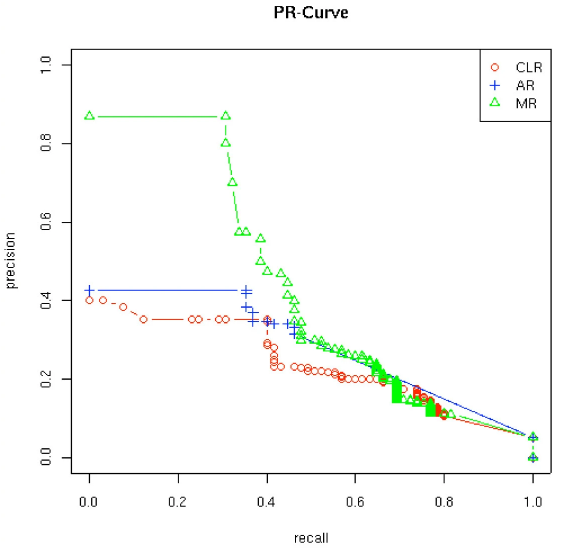
\includegraphics{https://raw.githubusercontent.com/Nertekkad/ml_nets/main/Images/Fig16.PNG}
\caption{\textbf{Figura 16:} Un gráfico de curvas PR (\emph{Precision-Recall curves}) que relaciona la precisión de cada algoritmo (CLR, ARACNE y MRNET), es decir, el valor predictivo de los modelos \([TP / (TP + FP)]\) con la recuperación o sensibilidad del modelo \([TP / (TP + FN)]\). Podemos observar que el poder predictivo de los modelos disminuye con el aumento de la sensibilidad, en otras palabras, la capacidad del modelo de predecir los valores de la nube de datos disminuye conforme este se vuelve más selectivo respecto a aquellos valores que el algoritmo considera pertinente medir, al tiempo que descarta aquellos que no. Imagen extraída de Meyer \emph{et al.}, 2008 \citep{meyer2008minet}.}
\end{figure}

Cabe destacar que si bien, los algoritmos previamente mencionados fueron diseñados para inferir redes de co-expresión de genes, al emplear el principio de co-abundancias para generar dichas redes también permite su potencial uso en la generación de redes ecológicas bacterianas.

Se han planteado numerosos métodos para la inferencia de redes ecológicas a partir bases de datos de microbiota, estos incluyen algoritmos de inferencia de matrices de similitud y disimilitud o distancias; por lo general empleando los coeficientes de correlación de Pearson o de Spearman \citep{chen2016two}. Ambos tipos de matrices son opuestos, pues mientras las primeras adquieren valores más altos entre mayor sea la correlación entre dos variables, las segundas lo hacen conforme aumenta la distancia entre las mismas. Sin embargo, por sí solos estos métodos carecen de la capacidad de diferenciar la presencia de correlaciones falsas, además de ser poco sensibles ante bajos números de muestra \citep{layeghifard2017disentangling}.

Debido a tales problemáticas se han planteado diversos modelos que buscan enfrentar las limitaciones de los primeros algoritmos. Podemos destacar el algoritmo SparCC (\emph{Sparse Correlations for Compositional data}), mismo que calcula las correlaciones lineales de Pearson a partir de haber aplicado previamente una transformación logarítmica a los datos, esto con el propósito de normalizarlos y reducir así la oblicuidad que pueda presentar su distribución \citep{friedman2012inferring}.

\[y_{ij} = log\frac{x_{i}}{x_{j}} = log(x_{i}) - log(x_{j})\]
El algoritmo asume previamente que el número de componentes, ya sean estos OTUs o genes, es alto; y que la mayoría de los componentes de la red no estarán fuertemente correlacionados, aunque el algoritmo es particularmente robusto a este último supuesto. A pesar de emplear la transformación logarítmica, el algoritmo no asume que los datos tengan estrictamente una distribución normal, sino que el uso de dicha transformación está motivado sencillamente por la facilidad que implica su implementación al procesar los datos. Esto tiene la ventaja de que el valor \(y_{ij}\) contiene información de las abundancias de los componentes, al ser una razón entre cada par de nodos, además de que esta relación es independiente del resto de OTUs de la base de datos. Cabe destacar que las correlaciones en este algoritmo pueden adoptar cualquier valor real y no se limitan a valores positivos (pues considera también correlaciones negativas potencialmente asociadas a relaciones antagónicas), razón por la cual se considera un umbral para seleccionar las conexiones entre nodos \citep{friedman2012inferring}. Cabe destacar que tanto la correlación de Pearson como la de Spearman asumen la linealidad de los datos, por lo que si la correlación entre dos nodos es no-lineal, el algoritmo asigna una correlación baja.

\begin{figure}
\centering
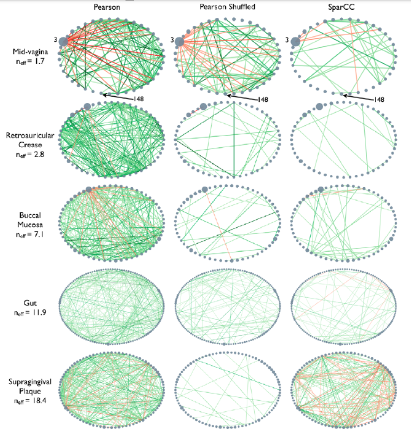
\includegraphics{https://raw.githubusercontent.com/Nertekkad/ml_nets/main/Images/Fig17.PNG}
\caption{\textbf{Figura 17:} Empleando datos de abundancias del 16S-rRNA extraídos del HMP, se construyeron redes empleando la correlación de Pearson, a la izquierda, y el algoritmo SparCC, a la derecha. También se emplearon datos estocásticos para una tercera red, en el centro. En verde se muestran las correlaciones positivas y en rojo las correlaciones negativas. El hecho de que la correlación de Pearson haya inferido conexiones a partir de los datos simulados podría indicar que algunas de las conexiones generadas con los datos reales mediante Pearson, podrían ser producto del sesgo inherente a los datos y no propiamente conexiones reales, además de que la distribución de las conectividades fue similar en ambos casos. Mientras tanto, el algoritmo SparCC no generó correlaciones significativas con los datos simulados, pero si con los reales. Imagen extraída de Friedman y Alm, 2012 \citep{friedman2012inferring}.}
\end{figure}

Otra metodología que ha sido empleada para la inferencia de redes ecológicas es SPIEC-EASI (\emph{SParse InversE Covariance Estimation for Ecological Association Inference}), que realiza dicha tarea aplicando primero una transformación de los datos originales para luego estimar el gráfico de la red seleccionandolos por vecindad (\emph{MB}) o por medio de la covarianza inversa (\emph{glasso}), permitiendo en ambos casos seleccionar las conexiones que se incluirán en la red \citep{kurtz2015sparse}. A diferencia de SparCC, que emplea como base la covarianza para estimar las conexiones, SPIEC-EASI se fundamenta en la independencia condicional, es decir, si en un par de nodos, ninguno de estos proporciona información adicional sobre el estado del otro, se les considera condicionalmente independientes; en cambio, sí así es y la correlación lineal entre sus abundancias no puede ser explicada sino es por la dependencia mutua, se les considera como nodos conectados \citep{meinshausen2006high}. El algoritmo es parsimonioso, privilegia aquellas condiciones donde los componentes aportan una mayor cantidad de información sobre sus parejas, descartando así las posibles correlaciones indirectas. El resultado es una red no-dirigida que considera únicamente correlaciones positivas entre los OTUs \citep{kurtz2015sparse}.

\begin{figure}
\centering
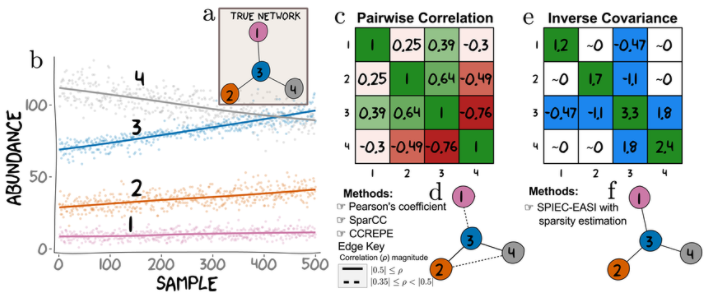
\includegraphics{https://raw.githubusercontent.com/Nertekkad/ml_nets/main/Images/Fig18.PNG}
\caption{\textbf{Figura 18:} En la imagen se simuló una base de datos de 500 muestras con distribución binomial (b) de acuerdo con una red prediseñada (a), para luego emplear distintos algoritmos para inferir dicha red a partir de los datos simulados (c, d), probando así la fiabilidad de cada uno de estos algoritmos en contraste con el método SPIEC-EASI (e, f). Algoritmos como SparCC, CCREPE o el coeficiente de Pearson permiten construir una matriz especular que considera tanto correlaciones positivas como negativas, sin embargo, el hecho de que requiera de un umbral arbitrario y de que este umbral sea seleccionado libremente por el investigador, provoca que el algoritmo sea susceptible a considerar como verdaderas correlaciones indirectas, especialmente si el umbral es lo suficientemente alto (c, d). En cambio, en el método SPIEC-EASI, mediante el uso de la covarianza inversa, la asociación depende de la condición como dependientes o independientes de los nodos pareados, asignando un valor de 0 a este último caso (e, f). Imagen extraída de Kurtz \emph{et al.} 2015 \citep{kurtz2015sparse}.}
\end{figure}

Como ya hemos mencionado, SPIEC-EASI puede emplear tanto la vecindad como la covarianza inversa para inferir la red. En el primer caso, el gráfico se construye a partir de comparar cada uno de los nodos por pares aplicando una regresión penalizada, mientras que en el segundo caso se emplea la máxima verosimilitud para analizar la independencia entre nodos \citep{bonneau2006inferelator}.

Si bien los algoritmos de coocurrencia se emplean a menudo para identificar interacciones entre especies, estos solo son capaces de inferir \emph{per se}, asociaciones ecológicas \citep{kurtz2015sparse}. Se considera que estos métodos son una herramienta útil para inferir potenciales interacciones entre taxones valiéndose del fundamento de que las poblaciones de cualquier organismo son dependientes de la abundancia de otros organismos, sin embargo, estas interacciones no suelen darse entre pocos organismos ni en condiciones controladas como sí ocurriría dentro de un laboratorio, sino que en un ecosistema microbiano podemos encontrar miles de taxones interactuando de distintas formas bajo condiciones variables \citep{hirano2019difficulty}. El caos y las dinámicas complejas inherentes a estos sistemas provocan que el uso de algoritmos, tales como SparCC y SPIEC-EASI, no puedan ser viables para identificar correctamente interacciones entre poblaciones de microorganismos, genes, etc \citep{kurtz2015sparse}. Si bien, se consideran herramientas útiles para inferir posibles asociaciones, no pueden ser consideradas como metodologías infalibles, aunado al hecho de que la aplicación de distintos algoritmos a distintas bases de datos suele presentar importantes discrepancias en los resultados que arrojan; razón por la cual deben ser entendidas como lo que son, herramientas de inferencia \citep{layeghifard2018constructing}. Para establecer una conexión entre los componentes de una red es importante obtener información extra que permita conocer la veracidad de la correlación, misma que se complementa con datos experimentales que permitan comprender si existe o no un mecanismo que conecte los componentes pareados y la naturaleza de dicho mecanismo \citep{hirano2019difficulty}.

\begin{figure}
\centering
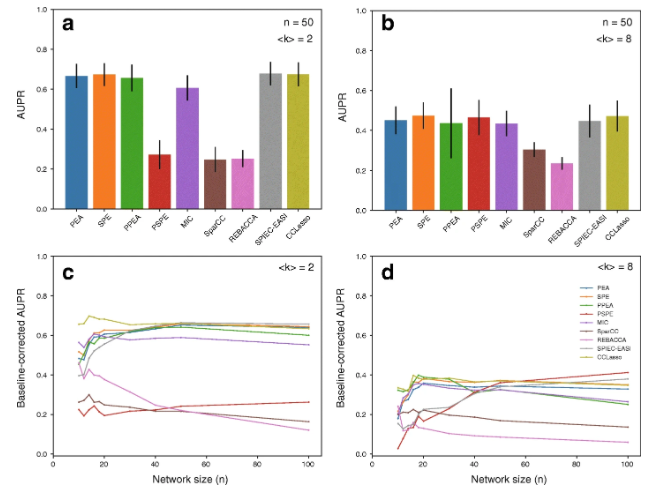
\includegraphics{https://raw.githubusercontent.com/Nertekkad/ml_nets/main/Images/Fig19.PNG}
\caption{\textbf{Figura 19:} Análisis de las discrepancias en los resultados obtenidos mediante distintos algoritmos de inferencia para una misma base de datos. Se consideró para ello una red con un total de 50 componentes y dos valores para el \emph{degree} promedio (\(〈k〉= 2m/n\)), donde n es el número de nodos y m el número de conexiones obtenidas. Se observa que los distintos algoritmos (a, b) presentan visibles diferencias entre los valores AUPR obtenidos (área bajo la curva PR, misma que relaciona la precisión de cada algoritmo con su sensibilidad). También podemos observar que algunos algoritmos son muy sensibles al tamaño de la red, y que a pesar de aumentar este parámetro las discrepancias entre los algoritmos no necesariamente disminuyen, por el contrario, pueden aumentar. Imagen extraída de Hirano y Takemoto, 2019 \citep{hirano2019difficulty}.}
\end{figure}

\hypertarget{la-microbiota-intestinal-y-su-impacto-en-la-salud-humana}{%
\section*{La microbiota intestinal y su impacto en la salud humana}\label{la-microbiota-intestinal-y-su-impacto-en-la-salud-humana}}
\addcontentsline{toc}{section}{La microbiota intestinal y su impacto en la salud humana}

La microbiota puede definirse como el conjunto de microorganismos (bacterias, hongos, arqueas, protozoos y virus) que proliferan y coexisten en los tejidos de un organismo multicelular. Los humanos tenemos una microbiota asociada a tejidos superficiales y cavidades; incluyendo el tracto digestivo, el tracto respiratorio, el tracto urinario, la piel, entre otras \citep{gamino2005flora}. Los microorganismos que componen la microbiota poseen complejas relaciones con el huésped, a menudo como comensales o simbiontes con un papel importante para el buen funcionamiento del organismo. Estas interacciones son dinámicas y al verse alteradas pueden tener un impacto sustancial en la salud del individuo. Diversos estudios epidemiológicos, ómicos y fisiológicos (tanto en modelos animales como en estudios en humanos) han revelado que la constitución de las comunidades microbianas tiene una influencia significativa como mediadores en el desarrollo de enfermedades en respuesta a estímulos ambientales \citep{fan2021gut}. Las alteraciones en respuesta a un estilo de vida poco saludable pueden provocar que los microorganismos con relaciones simbióticas con el huésped adquieran características patogénicas en respuesta a determinado estímulo, desencadenando un cuadro clínico. La microbiota ha probado tener un papel importante en la digestión, la regulación de la respuesta inmune, la función endocrina del intestino, la inactivación de toxinas, el metabolismo de fármacos y nutrientes, y la señalización neuronal, llegando a impactar incluso el estado emocional \citep{rothschild2018environment}.

Dada la inmensa diversidad de estilos de vida, patrones genéticos y epigenéticos, la gran variedad de taxones microbianos, y la complejidad inherente a la relación entre los tejidos y la microbiota asociada; establecer parámetros que delimiten una microbiota saludable de una que no lo es, resulta a menudo una tarea complicada. A pesar de ello, se toma como supuesto fundamental la composición y funcionamiento de la microbiota de individuos considerados sanos \citep{korem2015growth}. Para ello se toman como base las abundancias relativas de los microorganismos de interés, en lo concerniente a este documento, de las bacterias. Además, cabe destacar que el tipo de interacciones que presenta cierto grupo de microorganismos puede ser muy distinto de una especie a otra de una misma familia, o incluso de una cepa a otra de la misma especie, por lo que hacer generalizaciones al respecto puede resultar con frecuencia, contraproducente \citep{falony2018richness}. Por lo general, se considera que una microbiota más diversa está a menudo asociada a individuos sanos, pero la diversidad está también fuertemente ligada a la velocidad de tránsito intestinal, por lo que la diversidad y riqueza no pueden ser considerados como indicadores absolutos. Por ejemplo, un tránsito prolongado de la materia fecal puede contribuir a una mayor diversidad bacteriana, pero no necesariamente a una más saludable \citep{korem2015growth}.

Adquirimos nuestra microbiota durante el parto, cuando nuestro organismo es colonizado por millones de microorganismos distintos. A partir de este momento, la microbiota cambia gradualmente a lo largo de nuestra vida en respuesta a diversos estímulos que van desde el tipo de alimentación, la actividad física, la exposición a determinadas sustancias o la edad. El envejecimiento, por ejemplo, se ha asociado a una reducción en la diversidad microbiana en respuesta a cambios en la actividad del sistema inmune \citep{yatsunenko2012human}. Los microorganismos que componen la microbiota son los responsables de sintetizar metabolitos secundarios que tienen un impacto a distintos niveles en la fisiología del organismo, tales como la producción de ácidos grasos de cadena corta (AGCC), la síntesis de lipopolisacáridos (LPS), o la biosíntesis de vitaminas y aminoácidos esenciales \citep{qin2010human}. La fiabilidad de los datos metagenómicos debe ser sustentada con información complementaria, pues por si sola aporta una cantidad de información limitada a partir de la cual no es posible obtener conclusiones, sino que esta debe estar apoyada también en el entendimiento de los mecanismos que conectan los fenómenos observados con la diversidad microbiana \citep{backhed2004gut}.

Cabe destacar, también, que el uso masivo de antibióticos alrededor del mundo ha modificado sustancialmente los patrones de composición de la microbiota humana, y dado que casi la totalidad de humanos han estado expuestos a estos fármacos al menos una vez en su vida, se considera que existe un sesgo importante en la percepción de lo que consideramos como una microbiota core o central \citep{cox2015antibiotics}. De igual modo, los patrones dietéticos han sufrido importantes cambios en la mayoría de las sociedades desde la introducción de los alimentos pre-procesados, así como también modificaciones en el estilo de vida y la actividad física, el uso de probióticos y prebióticos, e intervenciones más radicales como la del uso de la fagoterapia o el trasplante de microbiota \citep{gorski2019perspectives}. Todos estos factores, en mayor o menor medida, constituyen un sesgo en la percepción del funcionamiento de la microbiota, más aún, considerando que la implementación de las tecnologías que nos permitieron aunar en la complejidad de tales sistemas es posterior a estos eventos. En los países desarrollados, donde muchos de estos fenómenos se han presentado con una mayor extensión en la población, se ha observado una reducción gradual de la diversidad microbiana. Esta reducción incluye géneros como \emph{Bacteroides}, \emph{Prevotella}, \emph{Desulfovibrio}, \emph{Lactobacillus} y \emph{Oxalobacter}, que ha su vez se ha asociado a una mayor prevalencia de enfermedades crónicas en contraposición con un aumento en los estándares de vivienda, seguridad alimentaria, acceso a servicios sanitarios e higiene \citep{clemente2015microbiome}. Dentro de esto podemos destacar la hipótesis de la higiene, misma que estipula que la exposición limitada a antígenos y patógenos relativamente comunes durante la infancia, ha dado paso a un desarrollo deficiente del sistema inmune, provocando que este reaccione de manera anómala ante estímulos ambientales cotidianos, siendo este fenómeno particularmente asociado a la aparición de alergias y enfermedades crónico-inflamatorias. Esta respuesta inmune anómala también conlleva alteraciones en la composición de la microbiota, alteraciones que permiten retroalimentar el estado crónico-inflamatorio de los individuos afectados \citep{smits2017seasonal}.

\begin{figure}
\centering
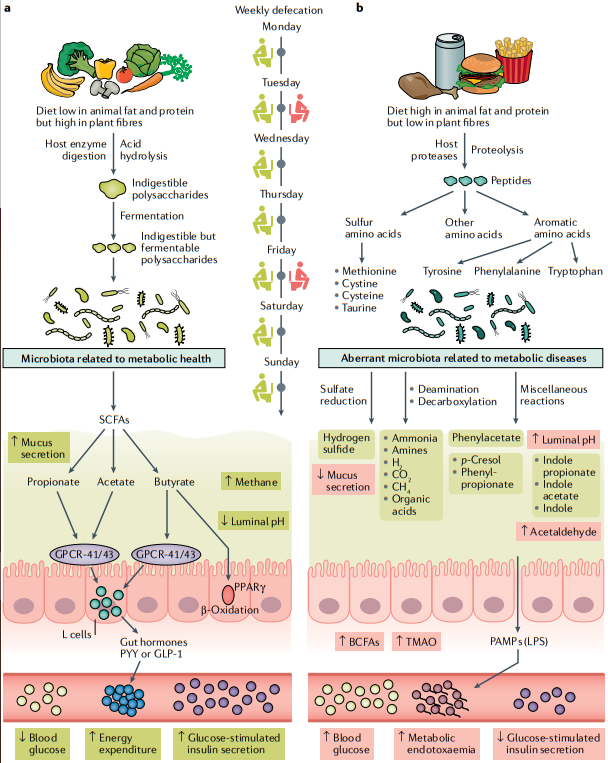
\includegraphics{https://raw.githubusercontent.com/Nertekkad/ml_nets/main/Images/Fig20.PNG}
\caption{\textbf{Figura 20:} El mantenimiento de la homeostasis depende de múltiples factores tanto ambientales como genéticos que, en su conjunto, afectan la composición de la microbiota. La disbiosis, como resultado de la alteración de las poblaciones microbianas, conduce a un estado de enfermedad. Una dieta rica en fibra y baja en grasas y proteínas animales conduce a la proliferación de bacterias fermentadoras de polisacáridos, mismos que son degradados a una variedad de compuestos que, entre otras cosas, promueven la producción de moco y la función de barrera del epitelio intestinal \citep{fan2021gut}. A partir de esta fermentación se obtienen ácidos grasos de cadena corta (AGCC), tales como el butirato, el propionato y el acetato; además del aumento en la producción de metano y la disminución del pH. Los AGCCs, además de ser una fuente de energía adicional para los colonocitos, interactúan con los receptores acoplados a proteínas G de las células L enteroendocrinas: GPCR-41 y GPCR-43, que a su vez inducen la secreción de péptido YY (PYY) y de péptido-1 similar al glucagón (GLP-1), que contribuyen a la sensación de saciedad, a la liberación de insulina y a el metabolismo de la glucosa \citep{flint2000effect}. Por su parte, el butirato favorece la beta-oxidación y el consumo de oxígeno en el intestino, ayudando a mantener un ambiente anaerobio, además de la regulación de la respuesta inmune mediante la estimulación de los linfocitos T reguladores \citep{maslowski2009regulation}. Por su parte, una dieta rica en proteínas y grasas animales, así como baja en fibra induce un estado de disbiosis, aunado a una vida sedentaria, una defecación infrecuente y el consumo recurrente de sustancias como el tabaco. Esta condición favorece la degradación de la mucosa por parte de las propias bacterias fermentadoras (en respuesta a la escasez de sustrato), la pérdida de la barrera intestinal y la filtración de compuestos de origen microbiano (PAMPs), incluyendo lipopolisacáridos (LPSs), al torrente sanguíneo, provocando un estado de inflamación que se ve agravado ante la baja producción de AGCCs \citep{macfarlane2006composition}. Esto también contribuye a retrasar la sensación de saciedad y altera el metabolismo de la glucosa al favorecer la resistencia a la insulina. Un tránsito lento aunado a un consumo rico en grasas y proteínas promueve igualmente un metabolismo proteolítico que conlleva el aumento de aminoácidos aromáticos, ácidos grasos de cadena ramificada, fenoles, indoles, gases y aminas, que contribuyen a aumentar el pH \citep{russell2013major}. Aunque, de igual modo, ha de notarse que la producción de indol y sus derivados a partir de la fermentación bacteriana de fibra favorece el metabolismo de la glucosa. Imagen extaída de Fan y Pedersen, 2021 \citep{de2017indolepropionic}.}
\end{figure}

La microbiota intestinal sufre cambios en individuos con obesidad. En las naciones occidentales la incidencia de obesidad ha aumentado en las últimas décadas, un fenómeno que se ha asociado al estilo de vida sedentario, alto consumo de alimentos ricos en grasas y azúcares, además del uso inadecuado y excesivo de antibióticos, que tienen un impacto en la composición de la microbiota. Se ha asociado a algunas especies productoras de ácidos grasos de cadena corta como \emph{Eubacterium ventriosum} y \emph{Roseburia intestinalis} con la obesidad \citep{tims2013microbiota}. Sin embargo, la síntesis de algunos tipos de AGCCs como el butirato, el propionato y el acetato por bacterias fermentadoras de fibra como \emph{Oscillospira} y \emph{Akkermansia muciniphila}, o arqueas como \emph{Methanobrevibacter smithii}, se han asociado al efecto contrario \citep{gophna2017oscillospira}. De igual modo, se ha asociado la presencia de bacterias fermentadoras de glutamato como \emph{Bacteroides thetaiotaomicron} con la delgadez, donde su abundancia es inversamente proporcional a la concentración sérica de glutamato \citep{miller1982isolation}. Además, la obesidad también se ha asociado con una reducción en la conjugación unidireccional, es decir, la transferencia de material genético entre bacterias, además de un aumento del estrés oxidativo derivado de una reducción de la actividad de las superóxido reductasas bacterianas, efectos que parecen ser reversibles mediante trasplantes de materia fecal en ratones \citep{ridaura2013gut}.

En individuos que padecen diabetes tipo II y prediabetes existe evidencia de una microbiota alterada con respecto a individuos sanos. Si bien esto no supone necesariamente que dicha alteración sea responsable de la resistencia a la insulina, la evidencia indica que la variación de las abundancias relativas si podrían tener un efecto indirecto sobre la secreción de insulina. Estudios en roedores indican que la hiperglucemia puede aumentar la permeabilidad de la barrera intestinal mediante la alteración de la actividad de GLUT2 en células epiteliales y el debilitamiento de las uniones estrechas, provocando una filtración de compuestos de origen bacteriano al torrente sanguíneo, lo que deriva en un estado de inflamación crónica \citep{thaiss2018hyperglycemia}. En individuos con prediabetes se ha identificado una considerable reducción en las abundancias relativas de taxones asociados a la síntesis de butirato, especialmente en el caso de \emph{Akkermansia muciniphila}, además de un aumento en poblaciones asociadas a la producción de factores proinflamatorios \citep{allin2018aberrant}. Cabe aclarar que el tratamiento farmacológico de la diabetes tipo II ha hecho difícil el estudio del papel de la microbiota en este padecimiento, debido a los factores de confusión derivados de los efectos que dichos fármacos puedan tener sobre las poblaciones microbianas. Por ejemplo, se ha documentado que la metformina altera las abundancias de diversos géneros bacterianos como \emph{Escherichia} e \emph{Intestinibacter}, aunque parece tener un impacto positivo en la producción de propionato y butirato, así como de ácidos biliares no-conjugados, induciendo así la gluconeogénesis intestinal y la consecuente reducción de la glucemia \citep{bryrup2019metformin}. Sin embargo, experimentos en roedores libres de gérmenes han indicado que los efectos de la metformina permanecen inalterados a pesar de la ausencia de una microbiota, lo que podría indicar que los efectos de dicho fármaco sobre la microbiota podrían ser más bien modestos \citep{adeshirlarijaney2019amelioration}. A pesar de la evidencia inicial, los cambios en la microbiota observados en individuos con diabetes tipo II parecen no ser específicos de dicha enfermedad, pues se han encontrado patrones similares también para el caso de otros trastornos crónicos caracterizados por una inflamación leve o clínicamente silenciosa. Además de que no se ha logrado reproducir con éxito el fenotipo de la diabetes al trasplantar materia fecal de ratones enfermos a ratones libres de gérmenes \citep{allin2018aberrant}.

Al desbalance o cambio en las abundancias relativas normales de los taxones bacterianos de la microbiota intestinal, se le conoce como disbiosis microbiana intestinal. La disbiosis se ha relacionado a un gran número de enfermedades cardio-metabólicas, siendo una de las más frecuentes la arteriosclerosis \citep{fan2016comprehensive}. Los individuos que padecen arteriosclerosis a menudo presentan concentraciones altas de glucosa sérica, insulina y lípidos, además de inflamación crónica de bajo grado y resistencia a la insulina, por lo que suele presentarse en personas que también padecen diabetes tipo II. Además, en casos más severos la arteriosclerosis también puede ir acompañada por cardiopatía isquémica, donde también se ha documentado los patrones de abundancias microbianas asociados a la disbiosis, Sin embargo, como igual sucede en el caso de la diabetes, el hecho de que las personas con arteriosclerosis estén fuertemente medicadas dificulta conocer cuál es el papel de la microbiota en el desarrollo de la enfermedad \citep{michos2019lipid}. Estudios realizados sobre muestras fecales de individuos con enfermedades cardio-metabólicas parecen exhibir abundancias enriquecidas de bacterias de la familia Enterobacteriaceae, tales como \emph{Escherichia coli}, \emph{Klebsiella spp.} y \emph{Enterobacter aerogenes}; en contraste con una disminución de \emph{Bacteroides spp.} y \emph{Faecalibacterium prausnitzii}. El cambio en dichas abundancias se ha correlacionado a un aumento en la síntesis de lipopolisacáridos, el transporte de aminoácidos, además de la síntesis de trimetilamina (TMA) y aminoácidos aromáticos como el triptófano. Por el contrario, existe una correlación inversa de la actividad de los AGCCs, especialmente de la producción del butirato, así como del metabolismo de vitaminas. En términos generales podemos aseverar que el microbioma se torna menos fermentativo al tiempo que promueve un estado de inflamación crónica leve \citep{sokol2008faecalibacterium}. Recientemente también se ha asociado una mayor abundancia de \emph{Ruminococcus}, \emph{Acinetobacter} y \emph{Veillonella spp.}, así como una disminución de \emph{Alistipes}, \emph{Faecalibacterium} y \emph{Oscillibacter spp.} como potenciales marcadores de la insuficiencia cardíaca isquémica \citep{cui2018metagenomic}.

La N-óxido de trimetilamina (TMAO) se ha identificado como un factor de especial relevancia en el desarrollo de enfermedades vasculares isquémicas. La trimetilamina (TMA) se sintetiza mediante la actividad enzimática bacteriana a partir de la fosfatidilcolina, la lecitina y la l-carnitina, compuestos abundantes en una dieta a base de productos cárnicos. Cuando la TMA ingresa al flujo sanguíneo del sistema porta enterohepático, viaja al hígado donde es oxidada a TMAO \citep{zhu2016gut}. Experimentos con roedores han mostrado que altas concentraciones séricas de TMAO provocan una aceleración del desarrollo de arteriosclerosis, aumentando la agregación plaquetaria y el riesgo de trombosis. Estudios con el inhibidor 3,3-dimetil-1-butanol de la síntesis de TMA han sido exitosos en reducir el riesgo de desarrollar arteriosclerosis, trombosis, infarto al miocardio, isquemia arterial y accidente cerebrovascular \citep{senthong2016intestinal}. Cabe destacar que existen inconsistencias en cuanto a los resultados, ya que experimentos con roedores alimentados con una dieta enriquecida con l-carnitina, si bien poseen concentraciones elevadas de TMAO como se esperaría, ver reducido al tamaño de las lesiones aórticas características de la isquemia vascular, por lo que la l-carnitina podría tener un efecto benéfico en contraposición a su condición como precursor de la TMA \citep{collins2016carnitine}. Sin embargo, estudios recientes en ratones sugieren que estas discrepancias podrían ser el resultado de una combinación de factores genéticos, la constitución de la microbiota y la dieta, que al interactuar entre sí predisponen al individuo en mayor o menor medida a desarrollar arteriosclerosis; por lo que si bien la concentración de TMAO puede ser útil como biomarcador, no supone necesariamente el desarrollo consecuente de la patología \citep{fan2021gut}.

La disbiosis intestinal también se ha relacionado al desarrollo de síndrome metabólico hepático, especialmente de hígado graso no-alcohólico (HGNA). El HGNA comprende un amplio abanico de enfermedades, siendo la esclerosis no-alcohólica la más agresiva de sus manifestaciones \citep{collins2016carnitine}. Pacientes con HGNA tienden a mostrar abundancias enriquecidas de \emph{Clostridium}, \emph{Anaerobacter}, \emph{Streptococcus}, \emph{Escherichia} y \emph{Lactobacillus}, al tiempo que presentan poblaciones reducidas de \emph{Oscillibacter}, \emph{Flavonifaractor}, \emph{Odoribacter} y \emph{Alistipes spp.} Las proteobacterias y enterobacterias parecen tener especial relevancia en el desarrollo de la enfermedad al verse aumentadas sus abundancias relativas. Dicha relación podría ser el resultado de compuestos hepatotóxicos sintetizados por la microbiota alterada, tales como 2-butanona y 4-metil-2-pentanona, se han hallado en concentraciones anormalmente altas en individuos con HGNA \citep{del2017gut}.

\begin{figure}
\centering
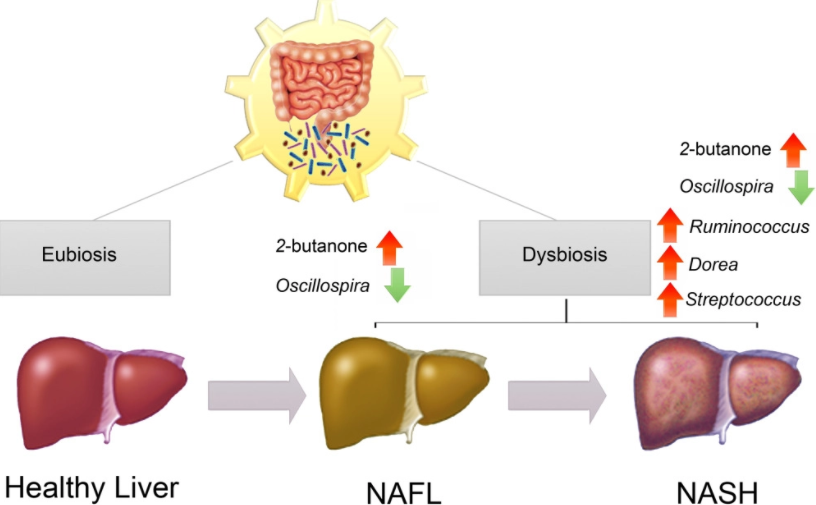
\includegraphics{https://raw.githubusercontent.com/Nertekkad/ml_nets/main/Images/Fig21.PNG}
\caption{\textbf{Figura 21:} La disbiosis microbiana intestinal se ha asociado al desarrollo de hígado graso no-alcohólico que puede incluso complicarse hasta convertirse en esteatohepatitis, es decir, hasta desarrollar un proceso necroinflamatorio del tejido hepático. La abundancia anormalmente alta de bacterias como \emph{Ruminococcus}, \emph{Dorea} y \emph{Streptococcus}, así como la disminución en las abundancias de \emph{Oscillospira}, se han propuesto como marcadores del desarrollo de este padecimiento, que podría asociarse a una mayor producción de compuestos hepatotóxicos como la 2-butanona por parte de la microbiota aberrante. Extraída de Del Chierico \emph{et al.}, 2017 \citep{del2017gut}.}
\end{figure}

Además, la mayor abundancia de bacterias productoras de etanol como \emph{Escherichia coli} contribuye también al desarrollo de la patología. El etanol es capaz de promover la actividad del factor nuclear κB (NF-κB), asociado a la respuesta a estrés y a la regulación de la actividad inmune, y cuya activación exacerbada es capaz de provocar daño tisular, contribuir a la endotoxemia en el sistema porta enterohepático y alterar la integridad de la barrera intestinal. Esto provoca un estrés añadido en el tejido hepático, que ve comprometida su capacidad de inactivar toxinas que a su vez contribuyen a retroalimentar el estrés oxidativo sobre los hepatocitos y el daño tisular, generando un estado de inflamación crónica del tejido hepático \citep{zhu2016gut}. Otras bacterias como Klebsiella pneumoniae parecen acelerar el desarrollo de la enfermedad, pero aún se requiere de una mayor investigación que ayude a esclarecer los mecanismos moleculares por los cuales la microbiota en general afecta el desarrollo de este tipo de patologías \citep{rao2004recent}.

Estudios sobre la microbiota de niños con desnutrición han arrojado indicios de cambios en la microbiota con respecto a individuos sanos. La microbiota sana en la infancia temprana se caracteriza por la floración temprana de bifidobacterias como \emph{Bifidobacterium longum} y \emph{Bifidobacterium pseudolongum}, responsables del metabolismo de la leche materna, cuyas poblaciones después se reducen en favor de la proliferación de bacterias anaerobias. Infantes con desnutrición aguda muestran una pérdida temprana de bifidobacterias, además de una escasa diversidad bacteriana en comparación con infantes sanos. Se ha señalado que la diversidad bacteriana se puede restablecer mediante una dieta equilibrada y suplementos vitamínicos, aunque no está del todo claro hasta qué punto esto es posible y los efectos sobre la microbiota a largo plazo \citep{smith2013gut}.

A pesar de que la información de la que disponemos actualmente no es suficiente como para comprender los mecanismos que conectan a la microbiota con el desarrollo de ciertas enfermedades, los estudios indican que se trata de una combinación de factores genéticos, ambientales y de la propia constitución de la microbiota, que en su conjunto dan lugar a un gran abanico de fenotipos. La propia definición de ``microbiota saludable'' resulta a menudo problemática debido en gran medida a la inmensa diversidad de estilos de vida y características individuales, haciendo que a menudo los datos muestran ciertas contradicciones en cuanto al difuso límite entre un estado de enfermedad y uno considerado como saludable. La compleja interacción entre las bacterias que componen la microbiota, el huésped y factores externos es aún un terreno desconocido, por lo que se requiere de mucha más investigación para comprender la relación entre tales factores y su papel en el desarrollo de patologías.

\hypertarget{uso-de-redes-en-la-exploraciuxf3n-de-la-microbiota}{%
\section*{Uso de redes en la exploración de la microbiota}\label{uso-de-redes-en-la-exploraciuxf3n-de-la-microbiota}}
\addcontentsline{toc}{section}{Uso de redes en la exploración de la microbiota}

La interacción entre las bacterias que componen la microbiota es aún en gran medida desconocida. Las poblaciones bacterianas responden a distintos factores que afectan la abundancia de las mismas bajo condiciones determinadas y en momentos determinados. Es así que, si bien pares de bacterias muestran interacciones que pueden ser simbióticas o antagónicas en condiciones experimentales, fuera de un medio controlado estas interacciones se pueden ver alteradas por las interacciones con otras bacterias, con el tejido del huésped y por los nutrientes derivados de la dieta del propio huésped y/u otros factores externos \citep{layeghifard2017disentangling}. Además podemos incluir la presencia de otras sustancias, tales como fármacos, otros organismos como parásitos, arqueas o bacteriofagos, y un gran número de variables, en su mayoría desconocidas, y que, como resultado de su efecto, afectan a las abundancias de las poblaciones \citep{falony2018richness}. Debido a la cada vez mayor evidencia sobre la importancia de la microbiota en el mantenimiento de la homeostasis, la comprensión de las relaciones inter-microbianas se ha tornado cada vez más relevante en el proceso de comprensión sobre el desarrollo de múltiples enfermedades \citep{rothschild2018environment}.

Por lo general, la microbiota se perfila mediante la amplificación y posterior secuenciación de genes marcadores como la región variable del 16S rRNA, cuyas lecturas suelen acoplarse en unidades denominadas OTUs (unidades taxonómicas operativas), o mediante la amplificación de segmentos de grandes regiones del ADN que incluyen múltiples genes mediante técnicas como la shotgun, que permiten alcanzar resoluciones a nivel de especie o incluso de cepa. Estas posteriormente se emplean para inferir las abundancias de cada uno de los taxones en función de la cantidad de material genético amplificado, y cuya concentración responde a la abundancia absoluta de cada OTUs en la muestra \citep{allin2018aberrant}. Estas secuencias son posteriormente clasificadas a distintos niveles taxonómicos, gracias a lo cual podemos agrupar los OTUs a nivel de género, familia, clase, \emph{phylum} y dominio. Las correlaciones altas entre dos OTUs sugieren una posible interacción entre ambos, si bien distintos algoritmos de inferencia de redes pueden mostrar resultados distintos al procesar los datos \citep{villaintroduction}. Debido a la co-ocurrencia de los OTUs, es posible identificar conjuntos o comunidades microbianas cuyos miembros están interconectados entre sí, lo que si bien no implica que interactúen directamente, si podría ser señal de que están relacionados de alguna manera o de que podrían estar involucrados en alguna actividad común, como por ejemplo la producción de AGCCs a partir de la fermentación de fibra dietética \citep{jackson2018detection}.

El algoritmo de co-ocurrencia WGCNA, desarrollado inicialmente para inferencia de redes de co-expresión génica, ha sido empleado también para la construcción de redes de la microbiota y la identificación de módulos de co-abundancia \citep{lozupone2012identifying}. El uso de redes como una de múltiples herramientas bioinformáticas en la exploración de la microbiota, contribuye a abordar la gran cantidad de datos obtenidos mediante la secuenciación y facilita la comparación de múltiples bases de datos en busca de patrones que puedan servir de punto de partida para comprender más a fondo las interacciones bacterianas \citep{guimera2005cartography}. La importancia funcional de las comunidades dentro de las redes es aún difusa, sin embargo la evidencia parece mostrar que comunidades o \emph{clusters} estrechamente interconectados son comunes en las redes microbianas, lo que sugiere que podrían tener una importancia biológica. Redes generadas mediante simulaciones por métodos bioinformáticos tienden a perder los \emph{clusters} típicamente encontrados con datos reales \citep{colizza2006detecting}. Dentro de estas comunidades los nodos con mayor \emph{degree}, que en teoría podrían corresponder a bacterias de especial relevancia dentro de la ecología de la propia microbiota, parecen estar mucho más interconectados que en el resto de la red. Además, también existe evidencia de que estas comunidades están relativamente conservadas entre individuos, aunque cabe destacar que distintos estudios también muestran discrepancias considerables en lo concerniente a este punto \citep{baldassano2016topological}.

\begin{figure}
\centering
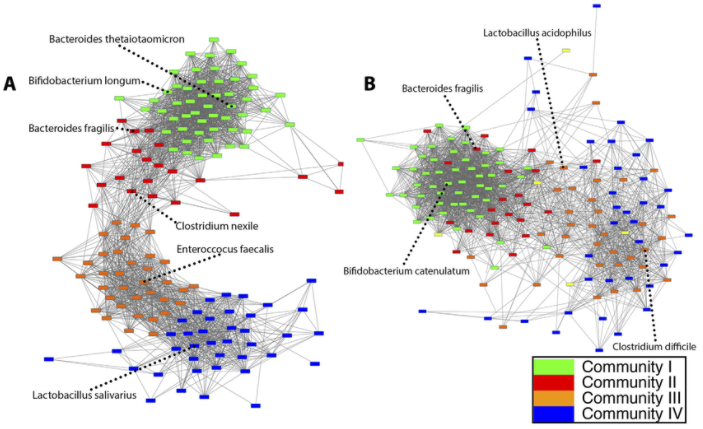
\includegraphics{https://raw.githubusercontent.com/Nertekkad/ml_nets/main/Images/Fig22.PNG}
\caption{\textbf{Figura 22:} Redes de microbiota inferidas mediante el algoritmo WGCNA. A la derecha se encuentra la red inferida a partir de datos de individuos sanos, y a la izquierda la red correspondiente a pacientes con síndrome de intestino irritable. El análisis de clusterización reveló que las comunidades encontradas corresponden a conjuntos de bacterias de distintas especies que potencialmente podrían tener una relación simbiótica. En la red de individuos sanos se encontraron 4 comunidades distintas en el 87\% de las iteraciones del algoritmo, mientras que en la red de individuos enfermos se encontraron 3 comunidades en el 99.9\% de las iteraciones. Mientras que en las comunidades de individuos sanos abundaban géneros como \emph{Bacteroides}, \emph{Bifidobacterium}, \emph{Prevotella}, y \emph{Ruminococcus}, asociados al metabolismo fibrolítico y a la síntesis de compuestos antiinflamatorios; en el segundo caso individuos abundaban géneros como \emph{Bacteroides} y \emph{Clostridium}, este último género está asociado al desarrollo de gastroenteritis. Imagen modificada de Smith \emph{et al.}, 2013 \citep{baldassano2016topological}.}
\end{figure}

A pesar de que las redes temporales y multiplex son herramientas relativamente recientes en la exploración de la microbiota, han probado ser de gran utilidad para comparar distintas redes. Como se ha mencionado previamente, un conjunto de bacterias no necesariamente interactúa de la misma forma bajo dos o más condiciones o periodos de tiempo distintos, por lo cual conocer en qué medida cambian las interacciones entre los nodos entre capas podría ayudar a comprender cómo la microbiota afecta y se ve afectada por los cambios ocurridos en su medio \citep{colizza2006detecting}. Las comunidades bacterianas no suelen permanecer estáticas ante variaciones en las condiciones de su medio, por ejemplo, durante el desarrollo de una enfermedad, en el proceso de envejecimiento, tras un cambio en la dieta o posterior a la ingesta de un fármaco. Debido a esto, algunas comunidades bacterianas tienden a ganar relevancia mientras otras la pierden, evento que tiene un impacto en la arquitectura de la red y que potencialmente puede ayudar a inferir la relevancia de las comunidades a nivel biológico \citep{guimera2005cartography}.

El uso de redes multicapa emerge como un nuevo paradigma de la teoría de redes, como una herramienta muy útil empleada en multitud de campos, incluída la biología. Este enfoque permite comparar redes heterogéneas y analizar las diferencias entre las mismas, la conservación de módulos entre capas y la identificación de diferencias en las propiedades de los nodos entre capas. Si bien posee numerosas limitaciones dentro del marco de sus posibilidades, es una herramienta útil que puede ayudar a reconocer patrones que podrían potencialmente tener relevancia en la dinámica del sistema biológico \citep{zheng2018improving}.

\begin{figure}
\centering
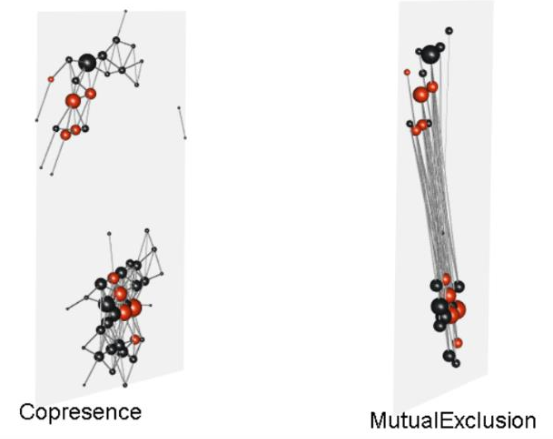
\includegraphics{https://raw.githubusercontent.com/Nertekkad/ml_nets/main/Images/Fig23.PNG}
\caption{\textbf{Figura 23:} Representación de la microbiota del rumen de bovinos donde se aislaron, a partir de una red original, dos comunidades específicas asociadas a la emisión de metano. Los nodos en rojo representan OTUs cuyas abundancias muestran diferencias significativas entre los individuos con alta y baja emisión de metano. Se construyó previamente una red de co-presencia, representando las interacciones mutualistas, y una de mutua exclusión, representando las interacciones antagónicas. Tal y como la hipótesis de los investigadores marcaba, no se identificaron conexiones compartidas entre ambas capas (debido a que una interacción no puede ser simultáneamente mutualista y antagónica). De igual modo, solo el 46\% de los nodos era compartido entre ambas capas. Los géneros \emph{Roseburia}, \emph{Pseudoramibacter}, \emph{Eubacterium} y \emph{Megasphaera}, mostraron abundancias más bajas en individuos de alta emisión que en el caso de los de baja emisión; además de que sus correspondientes nodos estaban altamente interconectado, lo que sugiere que cumplen un papel importante en la regulación de la emisión de metano. Imagen extraída de Zheng \emph{et al.}, 2018 \citep{zheng2018improving}.}
\end{figure}

\hypertarget{materiales-y-muxe9todos}{%
\chapter*{Materiales y métodos}\label{materiales-y-muxe9todos}}
\addcontentsline{toc}{chapter}{Materiales y métodos}

\begin{center}\rule{0.5\linewidth}{0.5pt}\end{center}

Se analizaron tres bases de datos tipo phyloseq bajo el enfoque de las redes multicapa. La primera de estas contenía datos de la microbiota del escarabajo Lema daturaphila y de la microbiota de la planta de la cual este se alimenta durante su estadio larval, la solanácea Datura inoxia \citep{mayoral2020extended}. También se analizaron dos bases de datos procedentes del paquete seqtime \citep{seqtime}, correspondientes a series temporales de la microbiota de dos sujetos; el primero de los cuales (sujeto A) realizó un viaje entre los días 71 y 122 durante los cuales cambió su régimen alimenticio, sufriendo en consecuencia dos episodios de diarrea entre los días 80 a 85 y 104 a 113. Por su parte, el sujeto B experimentó una intoxicación por \emph{Salmonella} entre los días 151 y 159 \citep{David2014}.

Para la realización de este trabajo se utilizó la versión 4.1.0 (2021-05-18) de R. Se emplearon los paquetes \emph{igraph} \citep{igraph}, \emph{phyloseq} \citep{phyloseq}, \emph{SpiecEasi} \citep{SpiecEasi}, \emph{minet} \citep{minet}, \emph{seqtime} \citep{seqtime}, \emph{muxViz} \citep{muxViz}, \emph{multinet} \citep{multinet}, \emph{corrplot} \citep{corrplot2021} y \emph{BiodiversityR} \citep{BiodiversityR}. Algunos de los paquetes están disponibles en CRAN y otros fueron descargados de repositorios de GitHub o del proyecto para análisis de datos genómicos Bioconductor.

\begin{longtable}[]{@{}llll@{}}
\toprule
\begin{minipage}[b]{0.24\columnwidth}\raggedright
Paquete\strut
\end{minipage} & \begin{minipage}[b]{0.15\columnwidth}\raggedright
Uso\strut
\end{minipage} & \begin{minipage}[b]{0.24\columnwidth}\raggedright
Fuente\strut
\end{minipage} & \begin{minipage}[b]{0.27\columnwidth}\raggedright
Descarga\strut
\end{minipage}\tabularnewline
\midrule
\endhead
\begin{minipage}[t]{0.24\columnwidth}\raggedright
igraph\strut
\end{minipage} & \begin{minipage}[t]{0.15\columnwidth}\raggedright
Construcción, diseño, análisis y manipulación de redes.\strut
\end{minipage} & \begin{minipage}[t]{0.24\columnwidth}\raggedright
CRAN\strut
\end{minipage} & \begin{minipage}[t]{0.27\columnwidth}\raggedright
install.packages(``igraph'')\strut
\end{minipage}\tabularnewline
\begin{minipage}[t]{0.24\columnwidth}\raggedright
phyloseq\strut
\end{minipage} & \begin{minipage}[t]{0.15\columnwidth}\raggedright
Herramientas para la importación, análisis, almacenamiento y la visualización de datos de microbioma.\strut
\end{minipage} & \begin{minipage}[t]{0.24\columnwidth}\raggedright
Bioconductor\strut
\end{minipage} & \begin{minipage}[t]{0.27\columnwidth}\raggedright
if(!requireNamespace(``BiocManager'', quietly = TRUE)) install.packages(``BiocManager''); BiocManager::install(``phyloseq'')\strut
\end{minipage}\tabularnewline
\begin{minipage}[t]{0.24\columnwidth}\raggedright
devtools\strut
\end{minipage} & \begin{minipage}[t]{0.15\columnwidth}\raggedright
Provee las funciones necesarias para el desarrollo de paquetes de R y descarga desde repositorios GitHub.\strut
\end{minipage} & \begin{minipage}[t]{0.24\columnwidth}\raggedright
CRAN\strut
\end{minipage} & \begin{minipage}[t]{0.27\columnwidth}\raggedright
install.packages(``devtools'')\strut
\end{minipage}\tabularnewline
\begin{minipage}[t]{0.24\columnwidth}\raggedright
SpiecEasi\strut
\end{minipage} & \begin{minipage}[t]{0.15\columnwidth}\raggedright
Estimación de la covarianza de datos de abundancia e inferencia de redes ecológicas.\strut
\end{minipage} & \begin{minipage}[t]{0.24\columnwidth}\raggedright
GitHub\strut
\end{minipage} & \begin{minipage}[t]{0.27\columnwidth}\raggedright
library(devtools); install\_github(``zdk123/SpiecEasi'')\strut
\end{minipage}\tabularnewline
\begin{minipage}[t]{0.24\columnwidth}\raggedright
seqtime\strut
\end{minipage} & \begin{minipage}[t]{0.15\columnwidth}\raggedright
Provee datos de series temporales de microbiota, y herramientas para simular y analizar la dinámica de comunidades microbianas en el tiempo.\strut
\end{minipage} & \begin{minipage}[t]{0.24\columnwidth}\raggedright
GitHub\strut
\end{minipage} & \begin{minipage}[t]{0.27\columnwidth}\raggedright
library(devtools); install\_github(``hallucigenia- sparsa/seqtime'')\strut
\end{minipage}\tabularnewline
\begin{minipage}[t]{0.24\columnwidth}\raggedright
muxViz\strut
\end{minipage} & \begin{minipage}[t]{0.15\columnwidth}\raggedright
Construcción, diseño y análisis de redes multicapa.\strut
\end{minipage} & \begin{minipage}[t]{0.24\columnwidth}\raggedright
GitHub\strut
\end{minipage} & \begin{minipage}[t]{0.27\columnwidth}\raggedright
devtools::install\_github(``manlius/muxViz'')\strut
\end{minipage}\tabularnewline
\begin{minipage}[t]{0.24\columnwidth}\raggedright
multinet\strut
\end{minipage} & \begin{minipage}[t]{0.15\columnwidth}\raggedright
Construcción, diseño y análisis de redes multicapa.\strut
\end{minipage} & \begin{minipage}[t]{0.24\columnwidth}\raggedright
CRAN\strut
\end{minipage} & \begin{minipage}[t]{0.27\columnwidth}\raggedright
install.packages(``multinet'')\strut
\end{minipage}\tabularnewline
\begin{minipage}[t]{0.24\columnwidth}\raggedright
corrplot\strut
\end{minipage} & \begin{minipage}[t]{0.15\columnwidth}\raggedright
Análisis de la correlación de matrices.\strut
\end{minipage} & \begin{minipage}[t]{0.24\columnwidth}\raggedright
CRAN\strut
\end{minipage} & \begin{minipage}[t]{0.27\columnwidth}\raggedright
install.packages(``corrplot'')\strut
\end{minipage}\tabularnewline
\begin{minipage}[t]{0.24\columnwidth}\raggedright
BiodiversityR\strut
\end{minipage} & \begin{minipage}[t]{0.15\columnwidth}\raggedright
Análisis de diversidad\strut
\end{minipage} & \begin{minipage}[t]{0.24\columnwidth}\raggedright
CRAN\strut
\end{minipage} & \begin{minipage}[t]{0.27\columnwidth}\raggedright
install.packages(``BiodiversityR'')\strut
\end{minipage}\tabularnewline
\bottomrule
\end{longtable}

\begin{figure}
\centering
\includegraphics{}
\caption{\textbf{Tabla 1:} Paquetes de R utilizados.}
\end{figure}

También desarrollé una serie de funciones en R que me permitieron analizar los datos, mismas que fueron almacenadas como un paquete de autoría propia que llamamos \textbf{ml\_BioNets}. Dicho paquete depende de \emph{igraph} \citep{igraph}, \emph{muxViz} \citep{muxViz} y \emph{phyloseq} \citep{phyloseq}.

\begin{longtable}[]{@{}lll@{}}
\toprule
\begin{minipage}[b]{0.35\columnwidth}\raggedright
Comando\strut
\end{minipage} & \begin{minipage}[b]{0.22\columnwidth}\raggedright
Uso\strut
\end{minipage} & \begin{minipage}[b]{0.35\columnwidth}\raggedright
Inputs\strut
\end{minipage}\tabularnewline
\midrule
\endhead
\begin{minipage}[t]{0.35\columnwidth}\raggedright
T\_collapse(T\_table, O\_table, names\_level)\strut
\end{minipage} & \begin{minipage}[t]{0.22\columnwidth}\raggedright
Suma las abundancias absolutas de los OTUs pertenecientes a cada uno de los clados del nivel taxonómico seleccionado.\strut
\end{minipage} & \begin{minipage}[t]{0.35\columnwidth}\raggedright
Tabla de taxones, tabla de OTUs y nivel taxonómico.\strut
\end{minipage}\tabularnewline
\begin{minipage}[t]{0.35\columnwidth}\raggedright
v\_colored(g, T\_table, g\_tax, p\_tax, g\_colors)\strut
\end{minipage} & \begin{minipage}[t]{0.22\columnwidth}\raggedright
Colorea los nodos en función del nivel taxonómico seleccionado. El resultado se almacena como un atributo asociado a los nodos al que llamamos \emph{color}.\strut
\end{minipage} & \begin{minipage}[t]{0.35\columnwidth}\raggedright
Red tipo igraph, tabla de taxones, nivel taxonómico superior, nivel taxonómico en el cual se infirió la red, y un carácter que contenga los colores que se asignados a cada clado.\strut
\end{minipage}\tabularnewline
\begin{minipage}[t]{0.35\columnwidth}\raggedright
g\_abundance(layer\_mat, g)\strut
\end{minipage} & \begin{minipage}[t]{0.22\columnwidth}\raggedright
Colorea los nodos en función de su abundancia relativa. El resultado se almacena como un atributo asociado a los nodos al que llamamos \emph{rel\_ab}.\strut
\end{minipage} & \begin{minipage}[t]{0.35\columnwidth}\raggedright
Matriz de abundancias de la capa y la red de la capa.\strut
\end{minipage}\tabularnewline
\begin{minipage}[t]{0.35\columnwidth}\raggedright
TaxGroup(g, T\_table, g\_tax, p\_tax)\strut
\end{minipage} & \begin{minipage}[t]{0.22\columnwidth}\raggedright
Indica a qué clado, de la categoría taxonómica seleccionada, pertenece un determinado grupo de nodos. El resultado se almacena como un atributo asociado a los nodos al que llamamos \emph{Taxon}.\strut
\end{minipage} & \begin{minipage}[t]{0.35\columnwidth}\raggedright
Red tipo igraph, tabla de taxones, nivel taxonómico superior, y nivel taxonómico en el cual se infirió la red.\strut
\end{minipage}\tabularnewline
\begin{minipage}[t]{0.35\columnwidth}\raggedright
ctr(g.list, ctr\_type)\strut
\end{minipage} & \begin{minipage}[t]{0.22\columnwidth}\raggedright
Colorea los nodos en un espectro de colores cálidos en función de su centralidad por grado, intermediación o cercanía. El resultado se almacena como un atributo asociado a los nodos al que llamamos \emph{hl}.\strut
\end{minipage} & \begin{minipage}[t]{0.35\columnwidth}\raggedright
Objeto muxViz y tipo de centralidad seleccionada (\emph{degree}, \emph{betweenness} o \emph{closeness}).\strut
\end{minipage}\tabularnewline
\begin{minipage}[t]{0.35\columnwidth}\raggedright
ctr\_g(g, ctr\_type)\strut
\end{minipage} & \begin{minipage}[t]{0.22\columnwidth}\raggedright
Colorea los nodos en un espectro de colores cálidos en función de su centralidad por grado, intermediación o cercanía. El resultado se almacena como un atributo asociado a los nodos al que llamamos \emph{hl}.\strut
\end{minipage} & \begin{minipage}[t]{0.35\columnwidth}\raggedright
Red tipo igraph y tipo de centralidad seleccionada (\emph{degree}, \emph{betweenness} o \emph{closeness}).\strut
\end{minipage}\tabularnewline
\begin{minipage}[t]{0.35\columnwidth}\raggedright
diff\_nodes\_graph(T\_Collapsed, n, mat\_list, g.list, alpha)\strut
\end{minipage} & \begin{minipage}[t]{0.22\columnwidth}\raggedright
Identifica diferencias significativas entre la media de las abundancias de nodos réplica en redes bipartitas. Esta función sólo considera los nodos con mayor abundancia. El resultado se almacena como un atributo asociado a los nodos al que llamamos \emph{colorA}.\strut
\end{minipage} & \begin{minipage}[t]{0.35\columnwidth}\raggedright
Tabla de abundancias de todas las muestras, número a nodos a considerar, lista de matrices de abundancias de las distintas capas, y el nivel de significancia alfa.\strut
\end{minipage}\tabularnewline
\begin{minipage}[t]{0.35\columnwidth}\raggedright
corr\_clusters(clusters, method, as.corrplot)\strut
\end{minipage} & \begin{minipage}[t]{0.22\columnwidth}\raggedright
Esta función permite generar una matriz de correlaciones de la clusterización entre las capas de la red, además de un gráfico de correlaciones.\strut
\end{minipage} & \begin{minipage}[t]{0.35\columnwidth}\raggedright
Lista de objetos tipo \emph{communities} para cada capa, generados con alguna de las funciones de clusterización de \emph{igraph}. Los métodos de comparación de la clusterización entre capas pueden ser ``\emph{vi}'', ``\emph{nmi}'', ``\emph{split.join}''. ``\emph{rand}'' o ``\emph{adjusted.rand}''. Si \emph{as.corrplot = T}, la función genera un gráfico de correlaciones, de lo contrario arroja una matriz de correlaciones.\strut
\end{minipage}\tabularnewline
\bottomrule
\end{longtable}

\begin{figure}
\centering
\includegraphics{}
\caption{\textbf{Tabla 2:} Funciones del paquete ml\_BioNets.}
\end{figure}

Previo a la inferencia de las redes, se colapsaron los datos a nivel de género en todas las bases de datos, eliminando previamente todos aquellos no-clasificados. Para esto se construyó la función \emph{T\_Collapse()}, que emplea como entrada la tabla de OTUs, la tabla de taxones y el nivel taxonómico hasta el cual se desea colapsar los datos. Dicha función suma las abundancias absolutas de los OTUs pertenecientes a cada uno de los clados dentro de la categoría taxonómica seleccionada.

Para inferir las redes se emplearon como datos de entrada una tabla de OTUs, que contiene las abundancias relativas de los OTUs en las muestras, y una tabla de taxones, misma que contiene la clasificación taxonómica de los OTUs. Para generar las redes multicapa previamente se separaron los datos concernientes a cada una de las capas. Para el caso de la red planta-insecto se separaron los datos correspondientes al escarabajo (huevos, intestino y excremento) y aquellos pertenecientes a la solanácea (endófitos, epifitos y semillas). Para los datos de series temporales, se separaron los períodos de salud y de enfermedad. Se aislaron tres secciones distintas de los datos del sujeto A, tomando en cuenta el periodo previo al viaje, durante el viaje y después del viaje. No fue posible construir redes únicamente a partir de los datos de los dos periodos de diarrea durante el viaje, debido a que el número de muestra era demasiado bajo como para que cualquiera de los algoritmos posteriormente utilizados pudiese inferir correlaciones entre los nodos. Para el sujeto B se tomó en cuenta el periodo previo a la infección por \emph{Salmonella}, el periodo durante el cual se desarrolló la infección, y el periodo posterior a esta.

Posteriormente se procedió a la inferencia de las redes para cada una de las capas, para lo cual se emplearon los algoritmos SparCC del paquete SpiecEasi \citep{SpiecEasi} y ARACNe del paquete minet \citep{minet}. Para el caso del algoritmo SparCC, se eliminaron todas las correlaciones por debajo de un umbral de 0.4. Inicialmente se planteó utilizar también el algoritmo SPIEC-EASI, pero debido a su alta selectividad, no fue posible construir redes para algunas de las capas con bajos números de muestra, razón por lo cual su uso se descartó. Se analizó también la diversidad de las distintas capas mediante los índices de Shannon y Simpson, además de la abundancia relativa de los \emph{phyla} en las capas. Se empleó el índice de diversidad de Rényi, también conocido como entropía de Rényi, mismo que cuantifica la insertidumbre del sistema en base al número de taxones y sus abundancias absolutas \citep{tothmeresz1995comparison}.

Para visualizar la distribución de los \emph{phyla} en la red se generó la función v\_colored(), que asigna un color a todos los nodos que pertenezcan a un mismo filo. Se construyó la función g\_abundance() con el fin de visualizar los nodos de la red en función de su abundancia relativa. Para analizar las características de la red también se analizó la distribución del \emph{degree} de las capas con una prueba de Shapiro-Wilk, y se comparó la distribución del \emph{degree} entre las capas.

El análisis de \emph{clusters} se realizó por el método \emph{Louvain}, mismo que optimiza la modularidad para detectar comunidades de nodos muy interconectados mediante el cálculo la densidad de aristas dentro de la red, cuyos valores pueden variar entre 1 y -1 \citep{combe2015louvain}. También se emplearon como complemento los métodos \emph{optimal} y \emph{fast-greedy}, para analizar la conservación de las comunidades encontradas bajo distintos algoritmos \citep{de2011generalized}. El primero maximiza la modularidad de todas las particiones posibles para calcular la estructura óptima de las comunidades del grafo \citep{klein1991optimal}, mientras que el segundo busca regiones con alta densidad de nodos y aristas en el grafo \citep{kazakovtsev2014genetic}. Se analizó la similaridad de los \emph{clusters} de las capas mediante el índice Rand, cuyo valor varía entre 0 y 1, y que toma en cuenta todos los pares de nodos posibles presentes y no presentes en el mismo \emph{cluster} en dos comunidades distintas, como ratio del número de pares desordenados posibles \citep{yeung2001details}. También se utilizó el coeficiente NMI (\emph{Normalized Mutual Information}), cuyo valor también oscila entre 0 y 1, que calcula la información compartida entre \emph{clusters} en función de los elementos compartidos, y considerando además la entropía como el número de clases de elementos distintos contenidos en un \emph{cluster} \citep{ana2003robust}.

\begin{figure}
\centering
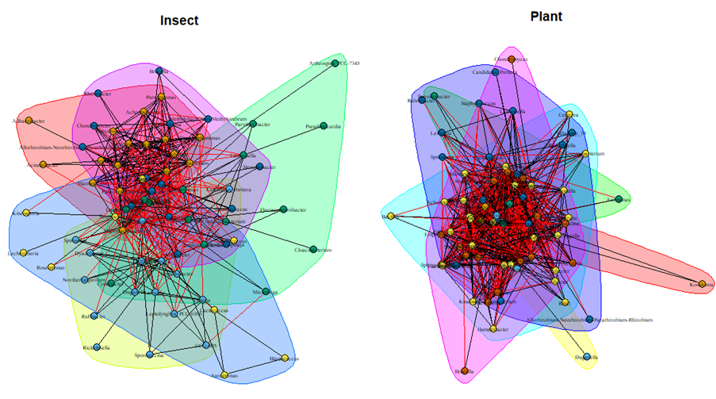
\includegraphics{https://raw.githubusercontent.com/Nertekkad/ml_nets/main/Images/Fig24.PNG}
\caption{\textbf{Figura 24:} Clusterización mediante el método \emph{Louvain} de las capas de la red escarabajo-solanácea. Los \emph{clusters} corresponden a regiones de la red ampliamente interconectadas. Las aristas que conectan los nodos dentro de la comunidad están representadas en negro, mientras que aquellas que conectan nodos entre comunidades distintas resaltan en rojo. Para facilitar la visualización de las comunidades se eliminaron los nodos cuyo \emph{degree} fuese nulo.}
\end{figure}

Se construyeron las redes multicapa utilizando el paquete \emph{muxViz}. La red escarabajo-solanácea se analizó bajo el enfoque de las redes multiplex, mientras que las redes de los sujetos A y B se analizaron como redes temporales. Se compararon los nodos de las comunidades entre las capas, para lo cual se utilizó la función TaxGruop(), que nos permitió identificar el \emph{phylum}, clase y familia a la que pertenecen los conjuntos de nodos clusterizados.

Se analizó la relevancia de los nodos de las comunidades mediante distintas medidas de centralidad, para lo cual se construyeron las funciones ctr() y ctr\_g() para redes multicapa y las redes simples, respectivamente. Solo se consideraron las centralidades por \emph{degree} e intermediación, debido a que la centralidad por cercanía no se definió correctamente ante la existencia de nodos y comunidades aisladas. Se identificaron nodos réplica con y sin diferencias significativas entre pares de capas mediante una prueba de t-Student (p\textless0.05). Únicamente se consideraron los 20 nodos con mayor abundancia dentro de las muestras. Finalmente, mediante el paquete \emph{multinet} \citep{multinet} se analizó la correlación entre capas con respecto a los nodos, el \emph{degree} y las conexiones en las redes temporales de los sujetos A y B.

\hypertarget{resultados}{%
\chapter*{Resultados}\label{resultados}}
\addcontentsline{toc}{chapter}{Resultados}

\begin{center}\rule{0.5\linewidth}{0.5pt}\end{center}

\hypertarget{resultados-de-la-red-escarabajo-solanuxe1cea}{%
\section*{Resultados de la red escarabajo-solanácea}\label{resultados-de-la-red-escarabajo-solanuxe1cea}}
\addcontentsline{toc}{section}{Resultados de la red escarabajo-solanácea}

De los tres algoritmos empleados en la inferencia de redes, solo ARACNe y SparCC fueron empleados en la construcción de las redes multicapa, descartando el uso de SPIEC-EASI para posteriores análisis. Este último está basado en la independencia condicional de los nodos, por lo cual es mucho más selectivo, y dado el bajo número de muestra de algunas de las capas, el algoritmo arroja redes inconexas para tales casos. El análisis de la distribución del degree de las capas reveló que esta se asemeja a una distribución normal. Cabe destacar que la interconectividad de la red del escarabajo realizada con ARACNe presentó una interconectividad considerablemente menor a la de su homóloga realizada con SparCC.

\begin{figure}
\centering
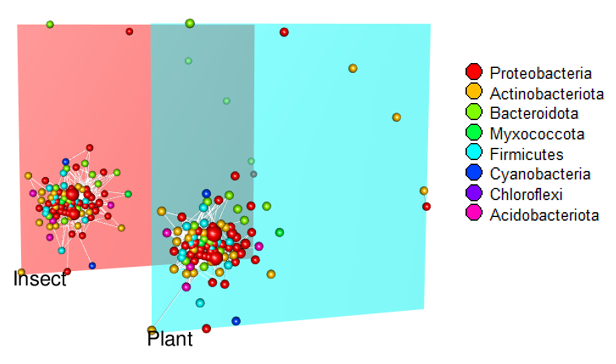
\includegraphics{https://raw.githubusercontent.com/Nertekkad/ml_nets/main/Images/Fig25.PNG}
\caption{\textbf{Figura 25:} Red multiplex (SparCC) de escarabajo-solanácea. El tamaño de los nodos está en función de la abundancia relativa de los nodos, cuyo color está asociado al \emph{phylum} al que pertenecen.}
\end{figure}

Las redes multicapa construidas con SparCC y ARACNe de escarabajo-solanácea, en ambos casos, revelaron a Proteobacteria como el \emph{phylum} con mayor abundancia y distribución en las capas. Del mismo modo, su abundancia relativa en las muestras de tejidos fue preponderante.

En las muestras extraídas del escarabajo se encontró una gran abundancia de las gamma-proteobacterias \emph{Serratia} y \emph{Pseudomonas}, pero una abundancia muy baja para el resto de OTUs presentes. La microbiota de la solanácea mostró una mayor diversidad de OTUs con abundancias altas, dentro de los que podemos destacar gamma-proteobacterias como \emph{Pseudomonas}, \emph{Pantoea}, \emph{Siccibacter}, \emph{Janthinobacterium} y \emph{Massilia}.

\begin{figure}
\centering
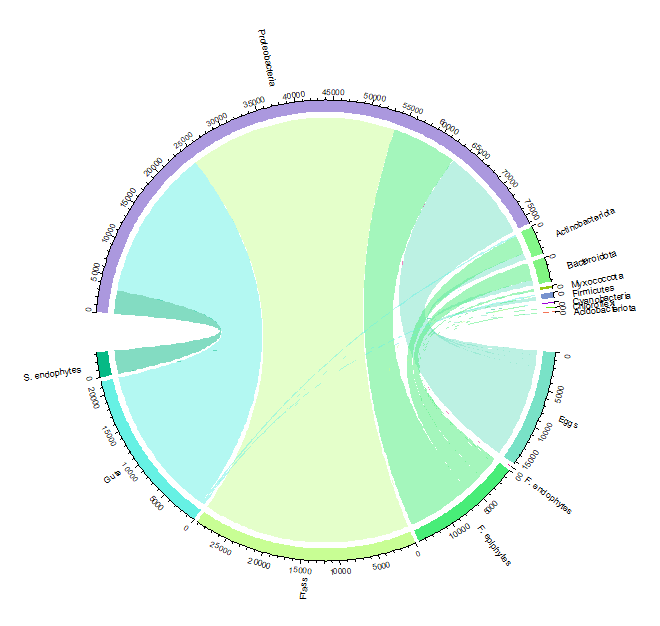
\includegraphics{https://raw.githubusercontent.com/Nertekkad/ml_nets/main/Images/Fig26.PNG}
\caption{\textbf{Figura 26:} Se analizó la distribución de los \emph{phylum} en las muestras de los distintos tejidos, mostrando una presencia dominante de Proteobacteria en todas las muestras, seguido en menor medida por Actinobacteria y Bacteroidetes.}
\end{figure}

Las muestras de excremento e intestino de \emph{Lema daturaphila} mostraron una diversidad de \emph{phyla} muy baja ante la abundancia dominante de Proteobacteria. Lo mismo sucede con las muestras endófitas extraídas de la planta. Las muestras con mayor diversidad fueron aquellas extraídas de los huevos del insecto y las muestras de epífitas de la solanácea, que también mostraron una presencia importante de Actinobacteria y Bacteroidetes, y en menor medida también de Firmicutes. Estas muestras, incluyendo las de excremento, obtuvieron valores superiores a 0.4 con el índice de Shannon, lo que indica una complejidad biológica superior a la del resto de muestras. Sin embargo, dichas muestras junto a las de intestino, mostraron valores cercanos a 1 en la diversidad de Simpson. Lo anterior significa que, si bien algunas muestras mostraron abundancias significativas de distintos taxones, la dominancia de las proteobacterias sigue siendo preponderante en las muestras.

El análisis de centralidades por \emph{degree} reveló que, a pesar de la variación de las abundancias entre ambos organismos, las Proteobacterias, conservan un alto grado de centralidad entre capas, lo que sugiere que podrían tener una importancia a nivel funcional en la relación entre el escarabajo y su fuente de alimento. Dentro de este grupo podemos destacar a \emph{Siccibacter} y \emph{Pantoea} en la microbiota del escarabajo, mismas que también mostraron previamente una abundancia relativa alta. El género \emph{Salmonella} también mostró un \emph{degree} alto en la red SparCC, aunque no se encontrara dentro de los OTUs con mayor abundancia relativa.

En el caso de la solanácea, la diversidad de especies con un \emph{degree} elevado fue mucho mayor. Destacan alfa-proteobacterias como \emph{Sphingomonas}, \emph{Skermanella}, \emph{Methylobacterium} y \emph{Microvirga}, además de gamma-proteobacterias como \emph{Janthinobacterium} y \emph{Massilia}. En menor proporción se encontraron también bacterias ajenas al \emph{phylum} Proteobacteria como \emph{Actinoplanes}, \emph{Hymenobacter} y \emph{Cystobacter}, pertenecientes a Actinobacteria, Bacteroidetes y Myxococcota, respectivamente.

\begin{figure}
\centering
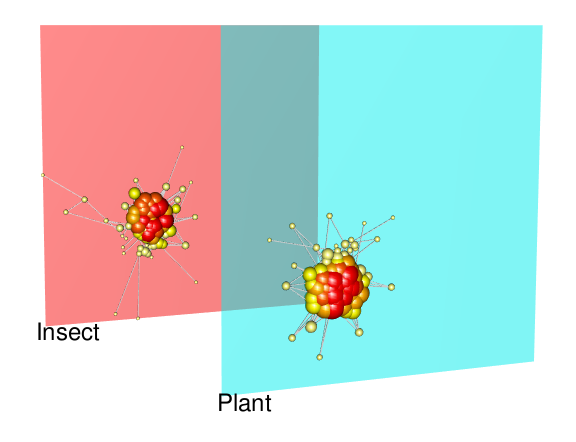
\includegraphics{https://raw.githubusercontent.com/Nertekkad/ml_nets/main/Images/Fig27.PNG}
\caption{\textbf{Figura 27:} Red multiplex de la centralidad por \emph{degree} entre las capas. Nodos con tonos más próximos al rojo indican un mayor número de conexiones.}
\end{figure}

El análisis de centralidad por cercanía mostró valores altos para casi todos los nodos debido a la alta interconectividad de los \emph{clusters}. Del mismo modo, no se encontró consenso al respecto de la centralidad por \emph{betweenness} entre los dos algoritmos.

\begin{figure}
\centering
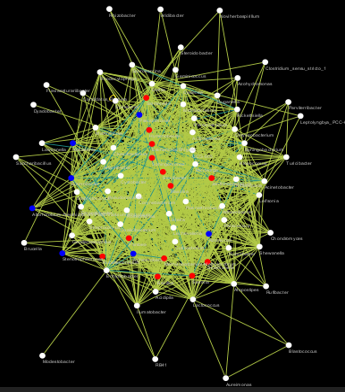
\includegraphics{https://raw.githubusercontent.com/Nertekkad/ml_nets/main/Images/Fig28.PNG}
\caption{\textbf{Figura 28:} Gráfico de la variación de los nodos entre las capas de la red bipartita. Los nodos marcados en rojo son aquellos que poseen diferencias significativas en las abundancias entre capas, mientras que los azules son aquellos que no poseen diferencias significativas entre ambas redes. Las conexiones representan la suma de interacciones en ambas capas.}
\end{figure}

No se encontraron diferencias significativas (p\textless0.05) en los géneros \emph{Kosakonia}, \emph{Stenotrophomonas}, \emph{Pseudomonas}, \emph{Azomonas}, \emph{Rhizobium}, \emph{Achromobacter} y \emph{Enterobacter}, todos pertenecientes al phylum Proteobacteria. Por el contrario, las proteobacterias \emph{Serratia}, \emph{Siccibacter}, \emph{Escherichia}, \emph{Shigella}, \emph{Pantoea}, \emph{Janthinobacterium}, \emph{Methylobacterium} y \emph{Salmonella}, además de \emph{Bacillus} de Firmicutes, se encontraron con mayor abundancia en los tejidos del escarabajo. Sin embargo, las proteobacterias \emph{Sphingomonas}, \emph{Massilia}, \emph{Rubellimicrobium} y \emph{Skermanella}, junto a \emph{Hymenobacter} de Bacteroidetes, tenían una abundancia mayor en los tejidos vegetales.

\hypertarget{resultados-de-las-redes-para-los-sujetos-a-y-b}{%
\section*{Resultados de las redes para los sujetos A y B}\label{resultados-de-las-redes-para-los-sujetos-a-y-b}}
\addcontentsline{toc}{section}{Resultados de las redes para los sujetos A y B}

Al igual que en el caso anterior, las redes fueron generadas únicamente con los algoritmos ARACNe y SparCC, pues no fue posible inferir las redes con SPIEC-EASI para la segunda capa de ambos sujetos debido a que, al tener un número de muestra bajo, el algoritmo no fue capaz de encontrar correlaciones entre sus componentes. La interconectividad de las redes generadas con ARACNe fue menor que en las redes generadas con SparCC. El análisis de la distribución del \emph{degree} en las redes ARACNe reveló que se trata de redes de mundo pequeño, donde la mayoría de las conexiones están concentradas en unos pocos nodos y la mayoría de los nodos tiene pocas conexiones. Ninguna de las redes SparCC presentó una distribución normal. En el caso de la diversidad Simpson como en la diversidad de Shannon, solo las muestras correspondientes a los periodos de enfermedad poseían una distribución normal en contraste con los estadios basales, lo que podría indicar un cambio en la dinámica de las poblaciones al presentarse la disbiosis.

Tanto en el sujeto A como en el sujeto B, la presencia de Firmicutes y Bacteroidetes era preponderante sobre el resto de \emph{phyla}, razón por la cual todas las muestras obtuvieron valores cercanos a la unidad en la prueba de diversidad de Simpson, en contraste con los valores bajos de diversidad de Shannon. En el sujeto A hubo un aumento significativo en la abundancia relativa de las proteobacterias en detrimento de Firmicutes, así como una reducción de Actinobacteria, durante el periodo de viaje. Durante el periodo de infección por \emph{Salmonella} en el sujeto B, también se registró un descenso en la abundancia relativa de Firmicutes, en contraste con un aumento en Bacteroidetes. Al igual que en el sujeto A, se identificó una reducción en la proporción de Actinobacteria. A pesar de que tras el periodo de infección hay un aumento de Firmicutes con respecto a Bacteroidetes, no se recuperan los valores previos y la abundancia relativa de Actinobacteria continúa siendo baja con respecto a sus valores iniciales.

\begin{figure}
\centering
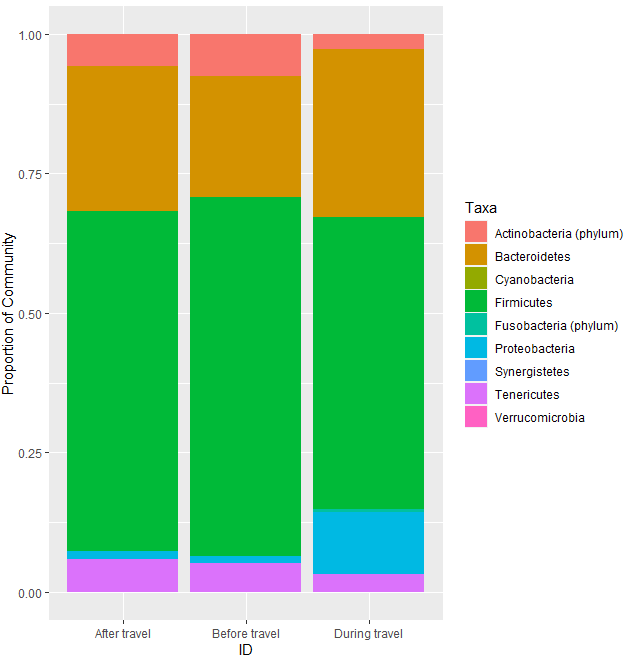
\includegraphics{https://raw.githubusercontent.com/Nertekkad/ml_nets/main/Images/Fig29.PNG}
\caption{\textbf{Figura 29:} Distribución de las abundancias de los \emph{phyla} en el sujeto A a lo largo de las tres capas, correspondientes al periodo previo al viaje, durante el viaje y posterior al viaje. Es durante el periodo de viaje en el cual el sujeto sufrió una alteración en la composición de su microbiota, derivada de un cambio en su dieta habitual.}
\end{figure}

En el sujeto A los géneros \emph{Bacteroides} y \emph{Faecalibacterium} se mantuvieron como los más abundantes en todas las capas. También se detectaron abundancias altas de \emph{Clostridium} y \emph{Blautia}. La abundancia de \emph{Bifidobacterium} decayó durante el periodo de disbiosis, aunque se recuperó después, a diferencia de las abundancias de \emph{Coprococcus}, cuya población no recuperó las abundancias iniciales. Durante la disbiosis se detectó un aumento considerable en las abundancias de \emph{Escherichia}, mismas que se redujeron tras el viaje. Por su parte, en el sujeto B, a pesar de tratarse de los dos géneros con mayor abundancia relativa, la presencia de \emph{Bacteroides} en las muestras fue mucho mayor que la de \emph{Faecalibacterium}. Si bien, las abundancias de ambos géneros se mantuvieron constantes, hubo un aumento en la abundancia relativa de \emph{Faecalibacterium} en el periodo post-infección. En las redes SparCC los géneros \emph{Bacteroides}, \emph{Faecalibacterium}, \emph{Clostridium} y \emph{Blautia} mantuvieron valores altos de centralidad por \emph{degree} en todas las capas de ambas redes temporales.

Las redes generadas con ARACNe presentaron comunidades con nodos altamente interconectados pero aislados del resto de nodos de la red, una particularidad que solo se presentó en las capas correspondientes a la disbiosis, en contraste con una mayor interconectividad de toda la red en las demás capas. La presencia de dichas comunidades se conservaron tras analizar el agrupamiento de las capas con los algoritmos \emph{Louvain}, \emph{optimal} y \emph{fast-greedy}. Cabe destacar que en el sujeto B, tras el periodo de disbiosis, la arquitectura de la red no se recuperó al encontrarse los nodos menos interconectados que al inicio del muestreo, en contraste con lo sucedido en el sujeto A.

En las redes ARACNe del sujeto A destacaban dos grandes comunidades altamente interconectadas en la capa de disbiosis. Ambas comunidades tenían una importante presencia de proteobacterias como \emph{Thauera}, \emph{Pseudoxanthomonas}, \emph{Brachymonas}, \emph{Polynucleobacter}, \emph{Rhodoplanes}, \emph{Massilia}, \emph{Methylotenera} y \emph{Rheinheimera}. Cabe destacar que las beta-proteobacterias fueron la clase más abundante en este grupo. Bacteroidetes también tuvo una presencia importante en dichas comunidades, destacando géneros como \emph{Hymenobacter}, \emph{Flavisolibacter}, \emph{Cytophaga} y \emph{Pedobacter}. Firmicutes también tuvo presencia con géneros como \emph{Alicyclobacillus}, \emph{Paenibacillus} y \emph{Caloramator}. Finalmente podemos mencionar la presencia de algunas actinobacterias como \emph{Rathayibacter}, \emph{Microcella} y \emph{Yonghaparkia}.

En los estadios basales del sujeto A, solo se encontraron comunidades pequeñas de entre tres y seis elementos. De la primera capa podemos destacar una comunidad formada por los géneros \emph{Rhizobium}, \emph{Erysipelothrix}, \emph{Williamsia}, \emph{Marinilactibacillus}, \emph{Cronobacter} y \emph{Providencia}. En la tercera capa no se encontraron comunidades mayores a cuatro elementos. Tales comunidades no se conservaron en las redes SparCC, donde la mayoría de los OTUs identificados como pertenecientes a las comunidades encontradas en las redes ARACNe, se hayaron como nodos aislados en las redes SparCC. La única excepción a esta regla fueron las comunidades de la segunda capa, cuyos elementos estaban integrados a comunidades de mayor tamaño en las redes SparCC.

En análisis de clusterización de las redes SparCC del sujeto A mostró grandes comunidades de bacterias, cuya composición se mantuvo similar a lo largo de todas las capas a pesar de los cambios en las abundancias relativas de las muestras. Géneros muy abundantes en las muestras como \emph{Bacteroides}, \emph{Faecalibacterium}, \emph{Clostridium} y \emph{Blautia} obtuvieron valores altos de \emph{degree}, lo que podría indicar que poseen una importancia destacable dentro de las comunidades encontradas. Cabe destacar que si bien, las comunidades encontradas tenían una presencia importante de Firmicutes y Proteobacteria, formando ambos grupos dos comunidades de gran tamaño, la presencia de Bacteroidetes, a pesar de su abundancia relativa alta en contraste con la mayoría de \emph{phyla}, fue marginal. Es importante destacar que a pesar de la reducción en las abundancias de Firmicutes y el aumento de Proteobacteria y Bacteroidetes durante el periodo de disbiosis, Bacteroidetes continuó teniendo una presencia marginal en las clusterizaciones encontradas.

Sin embargo, los algoritmos NMI y Rand empleados para analizar la correlación de la clusterización entre capas no arrojaron diferencias significativas, lo que podría estar asociado al gran número de nodos independientes presentes tanto en las redes SparCC como en las de ARACNe.

\begin{figure}
\centering
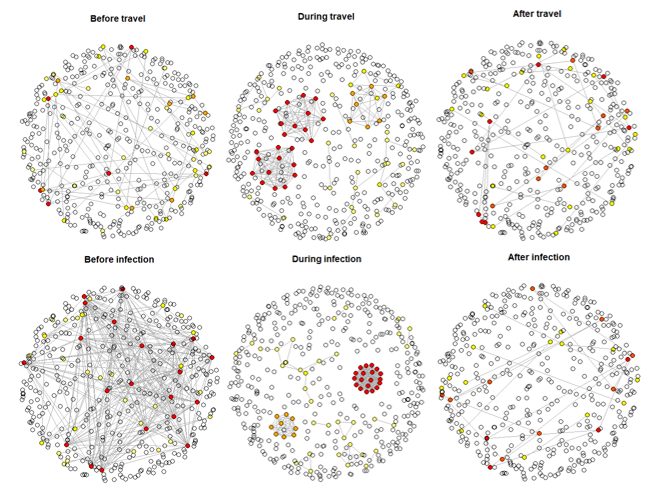
\includegraphics{https://raw.githubusercontent.com/Nertekkad/ml_nets/main/Images/Fig31.PNG}
\caption{\textbf{Figura 30:} Capas de las redes temporales de los sujetos A y B. Las regiones de la segunda capa de las redes ARACNe marcadas en rojo, corresponden a zonas con una alta densidad del \emph{degree}, donde fueron hayadas comunidades de bacterias altamente interconectadas compuestas principalmente por géneros de Firmicutes y Proteobacteria.}
\end{figure}

En el sujeto B, se identificó una reducción significativa en las abundancias de \emph{Bacteroides}, \emph{Actinobacillus}, \emph{Phascolarctobacterium}, \emph{Clostridium}, \emph{Streptococcus}, \emph{Oscillospira}, \emph{Alistipes} y \emph{Parabacteroides} en el sujeto A entre la primera y la segunda capa, en contraste con un aumento de \emph{Erwinia} durante el periodo de disbiosis. Las abundancias de dichos géneros recuperan sus proporciones originales tras el periodo de disbiosis. En el sujeto B el cambio en las abundancias fue mayor, especialmente entre la segunda y la tercera capa. De los géneros que se vieron modificados, podemos destacar a \emph{Bacteroides}, \emph{Hylemonella}, \emph{Actinobacillus}, \emph{Erwinia}, \emph{Phascolarctobacterium}, \emph{Clostridium}, \emph{Ruminococcus}, \emph{Coprococcus}, \emph{Eubacterium}, \emph{Faecalibacterium} y \emph{Akkermansia}. A diferencia de lo sucedido con el sujeto A, en este caso las abundancias de los géneros no solo no se recuperaron tras el periodo de disbiosis, sino que la mayoría de estos presentaron una abundancia incluso menor a la registrada durante el periodo de infección.

A pesar de la reducción de Firmicutes durante la infección por \emph{Salmonella}, la presencia de dicho \emph{phylum} fue destacable en los \emph{clusters} hallados en las redes ARACNe de la capa de disbiosis. Dentro de los géneros de Firmicutes identificados como pertenecientes a las comunidades del periodo de disbiosis, se incluyen \emph{Peptococcus}, \emph{Peptostreptococcus}, \emph{Facklamia}, \emph{Lachnospira}, \emph{Vagococcus}, \emph{Clostridium}, \emph{Blautia}, \emph{Ruminococcus}, \emph{Anaerostipes}, \emph{Eubacterium}, \emph{Weissella} y \emph{Faecalibacterium}. También destacó la presencia de proteobacterias como \emph{Vogesella}, \emph{Vitreoscilla}, \emph{Serratia}, \emph{Desulfovibrio}, \emph{Aquamonas}, \emph{Methyloversatilis}, \emph{Aquitalea} y \emph{Microvirgula}. La presencia de Bacteroidetes y Actinobacteria en tales comunidades, como también se observó en el sujeto A, fue marginal a pesar de la alta abundancia relativa de ambos \emph{phyla} en las muestras.

Si bien, la tercera capa del sujeto B mostró comunidades de bacterias pequeñas, tal y como también se observó en los estadios basales del sujeto A, en la primera capa se encontró una macrocomunidad compuesta por un gran número de géneros. Al igual que con las comunidades encontradas en las redes del sujeto A, la presencia de Proteobacteria y Firmicutres fue preponderante en todos los \emph{clusters}, un patrón presente tanto en las redes ARACNe como en las redes SparCC. Dentro de las proteobacterias halladas en los \emph{clusters} de la primera capa de las redes generadas por ambos algoritmos, destacamos los casos de \emph{Vogesella}, \emph{Vitreoscilla}, \emph{Serratia}, \emph{Desulfovibrio}, \emph{Methyloversatilis} y \emph{Aquamonas}. De los géneros pertenecientes a Firmicutes podemos destacar a \emph{Arcanobacterium}, \emph{Peptococcus}, \emph{Peptostreptococcus}, \emph{Facklamia}, \emph{Lachnospira} y \emph{Vagococcus}, mismos que también estuvieron presentes en los \emph{clusters} de la red SparCC. En ambos casos, en la tercera capa se encontraron comunidades de menor tamaño que las halladas en la primera capa, sin embargo, a diferencia del caso anterior no se encontró un consenso en cuanto a los elementos constituyentes de los \emph{clusters} hallados con ambos algoritmos. A pesar de ello, cabe destacar que tales comunidades contenían una presencia preponderante de Firmicutes y Proteobacteria. Al igual que en las redes del sujeto A, la presencia de Bacteroidetes en las comunidades del sujeto B fue marginal. Sin embargo, sí se encontró una presencia importante en todas las capas de Actinobacteria, destacando géneros como \emph{Arcanobacterium}, \emph{Rothia}, \emph{Microvirgula}, \emph{Bifidobacterium} y \emph{Varibaculum}, presentes en las comunidades halladas con ambos algoritmos. Tanto en las redes ARACNe como en las SparCC, en la segunda capa, referente al periodo de infección, se encontraron comunidades de mayor tamaño, comparadas con las capas del estado basal. Tales comunidades, sin embargo, presentaron una presencia importante de Firmicutes y Proteobacteria, como en los casos anteriores, además de una presencia considerablemente menor de Bacteroidetes.

Las alfa-proteobacterias mencionadas se hallaron agrupadas en un \emph{cluster} junto a otras bacterias como \emph{Hymenobacter}, \emph{Pseudomonas}, \emph{Janthinobacterium} y \emph{Massilia}. Además, todas las mencionadas se encontraron solo en las muestras de epífitas, lo que sugiere que forman una comunidad bacteriana cuyos miembros podrían tener funciones biológicas comunes. Sin embargo, la escasa diversidad de bacterias detectadas en las muestras de semillas y endófitas, también sugiere que el hecho de que la superficie de la planta podría simplemente ser un sitio más propicio para la proliferación de bacterias que los otros dos tejidos. Debido a ello, se requiere de un análisis mucho más exhaustivo que involucre agrupar los nodos por su función biológica para verificar si los \emph{clusters} realmente corresponden a comunidades relacionadas por su actividad biológica.

\hypertarget{discusiuxf3n}{%
\chapter*{Discusión}\label{discusiuxf3n}}
\addcontentsline{toc}{chapter}{Discusión}

\begin{center}\rule{0.5\linewidth}{0.5pt}\end{center}

\hypertarget{discusiuxf3n-de-la-red-escarabajo-solanuxe1cea}{%
\section*{Discusión de la red escarabajo-solanácea}\label{discusiuxf3n-de-la-red-escarabajo-solanuxe1cea}}
\addcontentsline{toc}{section}{Discusión de la red escarabajo-solanácea}

La relación de \emph{Lema daturaphila} y las especies del género \emph{Datura} es ampliamente conocida, puesto que dicho escarabajo es considerado como una plaga para múltiples especies de dicho género. A pesar de que \emph{Datura inoxia} sea una planta tóxica para la mayoría de insectos herbívoros, este escarabajo se ha adaptado para alimentarse de dicha planta solanácea. Las larvas del escarabajo se alimentan de las hojas de la planta durante el verano, y a menudo se les puede encontrar concentradas en grandes grupos en la superficie de las hojas \citep{goldberg2020towards}. Sin embargo, nuestro conocimiento sobre el papel de la microbiota en la relación entre ambas especies y su interacción con sus respectivos huéspedes, es aún muy limitado.

Todos los análisis revelaron una amplia presencia del \emph{phylum} Proteobacteria, un clado que sin embargo es muy diverso y, por lo tanto, difícil de asociar a una única función concreta. Su relación con la planta y el insecto varía a lo largo de un espectro muy amplio que incluye especies comensales, patógenas, simbiontes y bacterias de vida libre.

Dentro de este marco cabría señalar a las alfa-proteobacterias, algunas de las cuales suelen estar asociadas a tejidos vegetales como bacterias fijadores de nitrógeno, un papel que también desempeñan varias especies de beta-proteobacterias, clase que, sin embargo, no se encontró en proporciones significativas. Algunas de las alfa-proteobacterias identificadas, tales como \emph{Skermanella} y \emph{Microvirga}, se encuentran en una gran variedad de hábitats, especialmente en el suelo \citep{del2019soil}, lo que en primera instancia nos llevaría a plantear la hipótesis de que se trata de bacterias de vida libre. Sin embargo, el hecho de que estas se concentran casi exclusivamente en las muestras de epífitas sugiere una relación simbiótica o de comensalismo.

En el caso de \emph{Sphingomonas} y \emph{Methylobacterium}, ambos son géneros de bacterias fijadoras de nitrógeno, el primero de los cuales suele ser más abundante en las raíces de las plantas, mientras que en el género \emph{Methylobacterium} podemos encontrar simbiontes endófitas como \emph{Methylobacterium symbioticum}, y simbiontes epífitas como \emph{Methylobacterium extorquens} \citep{fausto2018olive}, aunque en las muestras analizadas solo se encontraron en las muestras de epífitas. Esto sugiere que la alta abundancia relativa de alfa-proteobacterias en las muestras, especialmente de \emph{Skermonella} debido a su sobresaliente presencia, podría estar relacionado con una asociación de tipo mutualista o comensal, como bacterias fijadoras de nitrógeno, con los tejidos superficiales de la solanácea.

Lo anterior contrasta con la mayor diversidad encontrada en las muestras del escarabajo. En dicho caso, la presencia de bacterias particularmente abundantes en heces e intestinos, como \emph{Serratia}, \emph{Pseudomonas}, \emph{Siccibacter}, \emph{Pantoea} y \emph{Salmonella}, también en muestras huevos, podría explicarse debido a que las larvas suelen cubrirse de excremento como mecanismo protector contra los depredadores \citep{visakorpi2021does}. Este fenómeno también podría explicar por qué se encontraron estas mismas bacterias en la superficie de la planta a pesar de estar fuertemente asociadas al intestino del escarabajo. Algunas de estas bacterias podrían estar involucradas en la digestión, pero también en la protección contra patógenos, como sucede con \emph{Serratia symbiotica} y su asociación con los áfidos, lo que le otorga a este último protección contra parásitos \citep{renoz2019evidence}. Esta hipótesis se ve fomentada ante el hecho de que \emph{Serratia} junto a \emph{Pseudomonas} son los géneros más abundantes en las muestras, y están ampliamente distribuidas en todos los tejidos analizados del insecto.

El análisis mediante redes multicapa identificó conjuntos de bacterias que podrían, dados los datos arrojados por los análisis, tener una función biológica importante en la regulación de la propia red y algunos incluso podrían actuar como simbiontes de sus huéspedes. Sin embargo, se requiere compaginar esta información con una base de datos de modo que podamos categorizar y etiquetar los nodos, e identificar si las funciones comunes asociadas a los OTUs se corresponden con los \emph{clusters} hallados.

\hypertarget{discusiuxf3n-de-las-redes-temporales-de-los-sujetos-a-y-b}{%
\section*{Discusión de las redes temporales de los sujetos A y B}\label{discusiuxf3n-de-las-redes-temporales-de-los-sujetos-a-y-b}}
\addcontentsline{toc}{section}{Discusión de las redes temporales de los sujetos A y B}

La microbiota intestinal humana es sumamente estable. A pesar de la constante variación en las abundancias de las poblaciones bacterianas a lo largo del tiempo, la mayor parte de estas poblaciones tiende a mantenerse dentro de un rango, independientemente de las constantes perturbaciones derivadas de la ingesta de alimentos, medicamentos, actividad física, entre otros factores involucrados \citep{costello2009bacterial}. Enfatizando lo anterior, un estudio de Caporaso \emph{et al.} (2011) calculó que alrededor del 95\% de los OTUs bacterianos encontrados en muestras de intestino y saliva, permanecieron en rangos estables a lo largo del periodo de muestreo, correspondiente a un año \citep{caporaso2011moving}. En general, a pesar de las constantes fluctuaciones en las poblaciones bacterianas a lo largo de una serie de tiempo, estas tienden a aproximarse a determinados valores de equilibrio que dependen en gran medida de sus interacciones con otros OTUs bacterianos, lo que mantiene la estabilidad de las comunidades. Sin embargo, la exposición prolongada y sostenida a un agente perturbador, como puede ser un antibiótico, si promueve cambios importantes en la dinámica de las poblaciones a largo plazo \citep{dethlefsen2011incomplete}.

El estudio realizado por David \emph{et al.} (2014) mediante el enfoque de las series temporales, reveló que, en el periodo de viaje durante el cual el sujeto A vio modificado su régimen alimenticio, la dinámica de las poblaciones bacterianas se vio alterada significativamente. Sin embargo, tras dicho periodo, y luego de que el sujeto A retomara su dieta habitual, la dinámica de poblaciones se restableció a un estado similar al registrado previamente al viaje. En contraste, en el sujeto B un fenómeno similar se observó durante el periodo de infección por \emph{Salmonella}, sin embargo, a diferencia del primer caso la dinámica de la microbiota no se recuperó, y se reportó una considerable pérdida de la diversidad \citep{david2014host}.

\begin{figure}
\centering
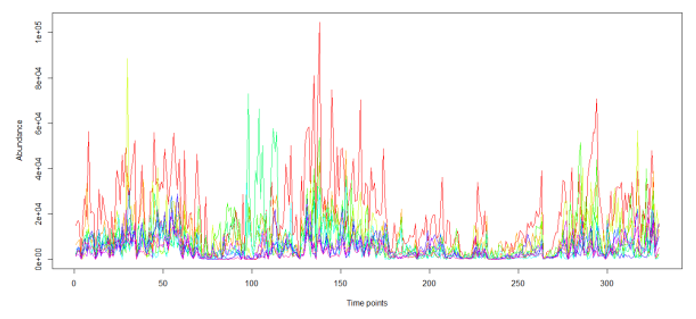
\includegraphics{https://raw.githubusercontent.com/Nertekkad/ml_nets/main/Images/Fig32.PNG}
\caption{\textbf{Figura 31:} Serie temporal de los diez OTUs más abundantes en las muestras del sujeto A, mismo que sufrió un cambio en la dinámica de su microbiota derivado de un viaje realizado entre los días 71 y 122, durante los cuales modificó su dieta habitual.}
\end{figure}

El cambio en la distribución tanto del \emph{degree}, en las redes ARACNe, como en la distribución de la diversidad en los periodos de disbiosis en contraste con los estadios basales, podría ser un indicativo de una alteración en la dinámica habitual de las poblaciones bacterianas. Sin embargo, en las redes SparCC del sujeto A, la evidencia en cuanto a un cambio en la interconectividad y los \emph{clusters} encontrados en la red no arrojó resultados concluyentes, a pesar de las alteraciones en las abundancias encontradas en las muestras. Sin embargo, el cambio en la arquitectura de las redes ARACNe, especielmente en lo referente a las comuniades bacterianas hayadas en periodos de disbiosis en contraste con los periodos basales, sugiere una posible alteración de las interacciones entre los OTUs bacterianos que potencialmente podrían contribuir a entender el papel de la microbiota en periodos de enfermedad y como esta misma microbiota se ve alterada en tales períodos.

Si bien en el sujeto B, tanto las abundancias como la arquitectura de la red ARACNe no parecen recuperarse tras el periodo de disbiosis, la ausencia de datos posteriores no permite descartar la posibilidad de que la microbiota del sujeto B no se haya recuperado en los días posteriores, o si realmente la infección por \emph{Salmonella} derivó en cambios significativos que perdurasen a largo plazo.

En ambos casos se encontró una alteración en el ratio Bacteroidetes/Firmicutes (B/F), reflejándose una reducción de la abundancia relativa de Firmicutes en detrimento de Bacteroidetes y de otros \emph{phyla}, como es el caso de Proteobacteria en el sujeto A. La importancia de los \emph{phyla} Firmicutes y Bacteroidetes en la microbiota humana es bien conocida, pues constituyen alrededor del 90\% de la diversidad microbiana intestinal \citep{magne2020firmicutes}. Esto ayudaría a explicar los valores altos en el índice de Simpson de todas las muestras, pues se trata de un índice de dominancia cuyos valores se incrementan en presencia de taxones con abundancias relativas predominantes en comparación con el resto de las poblaciones \citep{indiani2018childhood}. Si bien, la abundancia de estos dos \emph{phyla} puede variar entre individuos dependiendo de sus características fisiológicas, su estilo de vida, alimentación o factores genéticos, se considera que un aumento en la abundancia relativa de Bacteroidetes en detrimento de las poblaciones de Firmicutes está asociado al síndrome de intestino irritable. El caso contrario se ha relacionado con la obesidad \citep{magne2020firmicutes}. En el caso de los sujetos A y B, la alteración del ratio B/F podría estar asociada al proceso inflamatorio derivado de un proceso infeccioso \citep{stojanov2020influence}. Si bien en el sujeto B se conoce que sufrió una intoxicación por \emph{Salmonella}, en el sujeto A el proceso podría estar asociado a un aumento puntual de la abundancia de \emph{Escherichia} durante el periodo de disbiosis. Esta hipótesis se ve reforzada ante el hecho de que en las redes SparCC, \emph{Escherichia} adquiriera una mayor grado o \emph{degree} dentro de las redes.

Los \emph{phyla} Proteobacteria y Actinobacteria son, después de Firmicutes y Bacteroidetes, de los grupos más abundantes e importantes en la microbiota intestinal humana. Se ha documentado que un incremento de proteobacterias está asociado a la disbiosis y al decremento en la abundancia de Firmicutes en individuos con enfermedad inflamatoria intestinal \citep{magne2020firmicutes}, un fenómeno que coincide con las observaciones de los sujetos A y B, donde ambos estuvieron expuestos a un proceso inflamatorio. También se ha asociado que el incremento de Proteobacteria está correlacionado con el decremento de la abundancia de Actinobacteria \citep{stojanov2020influence}, como se pudo observar en las muestras del sujeto A. También podemos destacar que la alteración en la abundancia de bacterias como \emph{Bifidobacterium} o \emph{Coprococcus} en ambos sujetos durante el periodo de disbiosis, podría estar asociado al desarrollo de un proceso inflamatorio derivado de la infección, pues ambos géneros están asociados a la producción de ácidos grasos de cadena corta, mismos que juegan un papel importante en la regulación de la actividad inflamatoria \citep{lee2018blueberry}.

Si bien, en las redes SparCC la evidencia no fue concluyente como para asegurar un cambio significativo en la arquitectura de las redes, y por lo tanto, de las comunidades de bacterias encontradas, el hecho de que tanto las abundancias como la arquitectura de las redes ARACNe adoptaran configuraciones similares a las encontradas en el periodo previo a la infección, sugiere que el sistema en su conjunto, a pesar de verse alterado durante periodos de infección, es robusto ante perturbaciones. Cabe destacar que el hecho de que las comunidades de las redes SparCC, ricas en Firmicutes y Proteobacteria, se hayan mantenido en el tiempo a pesar de las alteraciones en las abundancias derivadas de la disbiosis en los sujetos, refuerza la hipótesis de que el sistema parece ser robusto ante perturbaciones, y que ambos \emph{phyla} están ampliamente relacionadas entre sí y juegan un papel importante en el mantenimiento de la microbiota, aunque se requiere de un análisis más profundo para sustentar esta aseveración.

\hypertarget{conclusiones-generales}{%
\section*{Conclusiones generales}\label{conclusiones-generales}}
\addcontentsline{toc}{section}{Conclusiones generales}

El uso de redes multicapa se postula como una herramienta útil en el análisis de la microbiota debido a que permite comparar las propiedades y la arquitectura de distintas redes, ya sea que estas representan segmentos en una escala temporal, como vimos con la evolución de la microbiota a lo largo de un proceso infeccioso, o el estado de la microbiota bajo dos regímenes distintos, como pudimos estudiar cuando comparamos la microbiota de dos organismos estrechamente relacionados en la cadena trófica. Esto nos permite identificar y estudiar patrones que no serían posibles de analizar limitándose a la implementación del enfoque tradicional de la teoría de redes.

Sin embargo, cabe destacar que el hecho de que existan importantes discrepancias en cuanto a la inferencia de redes a partir del uso de distintos algoritmos, indica que si bien las redes de coabundancia pueden ser útiles como herramientas para analizar la posible existencia de interacciones entre microorganismos, sus resultados deben ser tomados con cautela. A lo largo del presente trabajo nos limitamos a emplear datos de abundancias de los distintos OTUs encontrados en las muestras, lo que plantea importantes limitaciones en cuanto a conocer la naturaleza de las interacciones entre los organismos y su potencial funcionalidad dentro del sistema. Combinar estas técnicas con otras herramientas, como puede ser el uso de series temporales o de redes de redes que combinan los datos existentes con información sobre los metabolitos secundarios producidos por los microorganismos en cuestión, permitiría ampliar nuestra comprensión, no solo sobre la forma en que los microorganismos interactúan entre sí, sino también sobre cómo afectan a los tejidos del hospedero.

\hypertarget{referencias}{%
\chapter*{Referencias}\label{referencias}}
\addcontentsline{toc}{chapter}{Referencias}

  \bibliography{book.bib}

\end{document}
